\chapter{Architecture}
\label{chap:architecture}


\begin{chapterintro}
This chapter describes in depth how the system is structured in different modules and how the users interact with them and also how the modules interact with other modules by themselves.
\end{chapterintro}

\cleardoublepage
\section{Architecture Overview}
In this section we will describe the \textbf{videogame architecture}, starting with its two main modules, the \textbf{physical instruments miniatures} and the \textbf{software application}. In Figure \ref{fig:ArchitectureGeneral} we show the global game architecture identifying both main modules and their relation.

\begin{figure}[ht!]
	\centering
	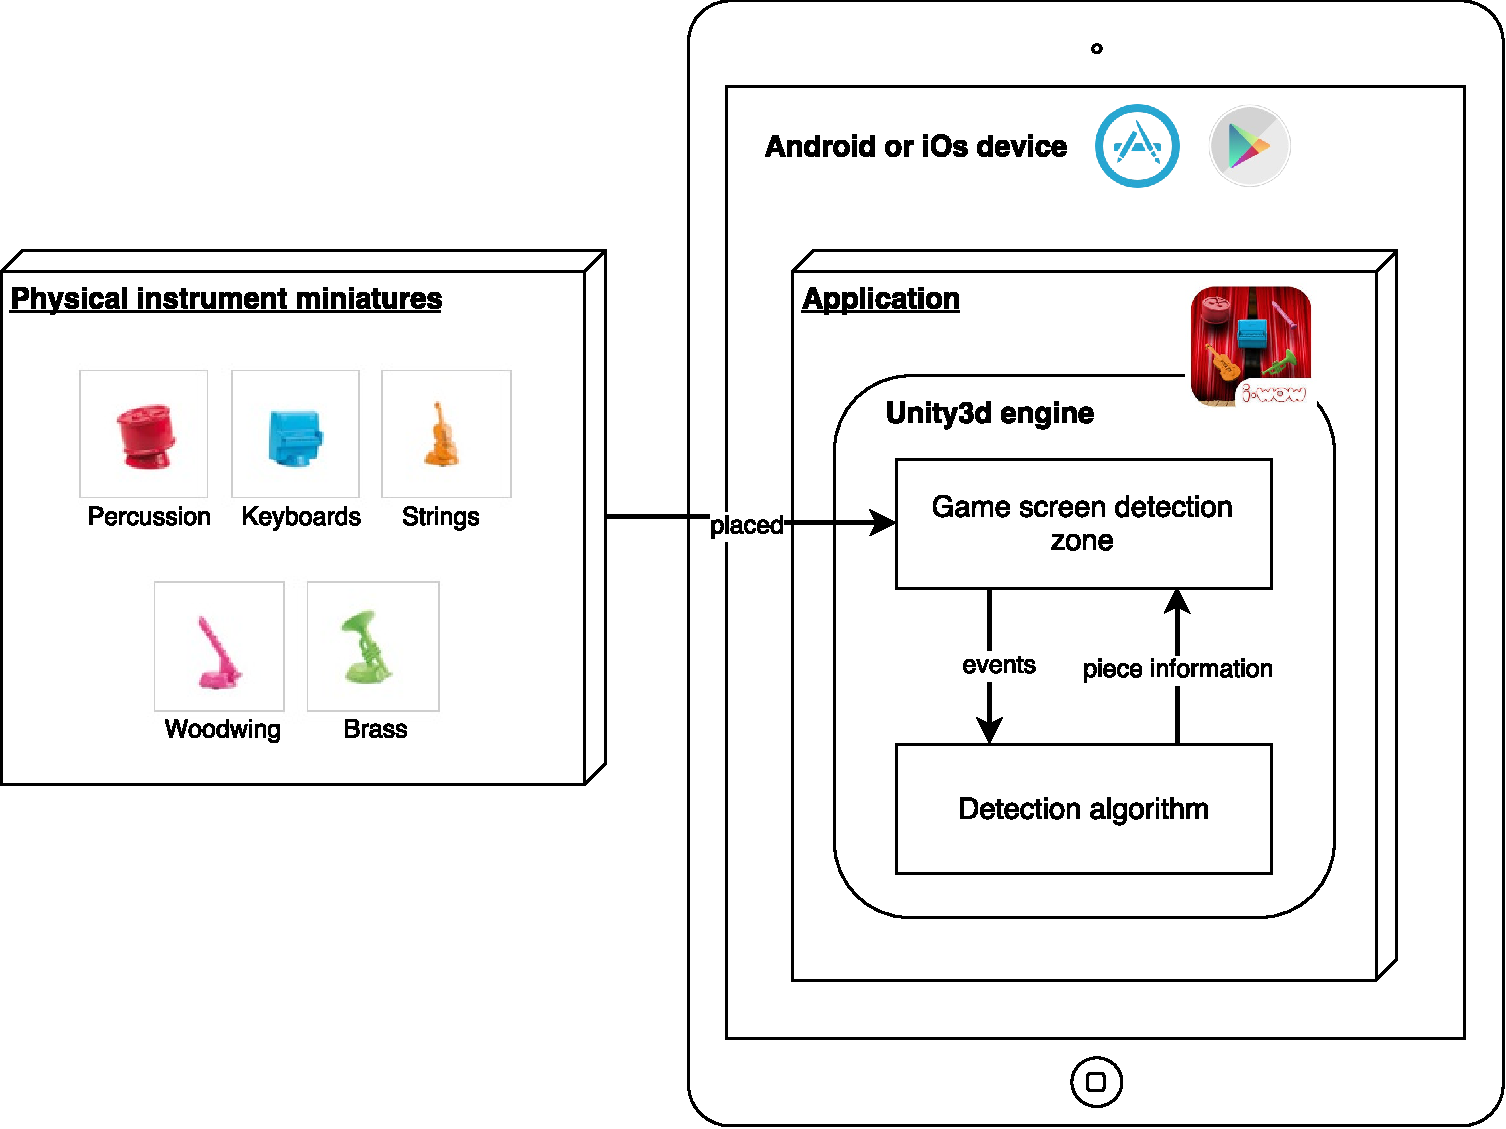
\includegraphics[width=400pt]{graphics/architecture/ArchitectureGeneral.pdf}
	\caption{General Architecture}
	\label{fig:ArchitectureGeneral}
\end{figure}

\FloatBarrier

The modules are detailed below.

\subsection{Physical instruments miniatures}
There are five physical miniatures which represent each one of the musical instrument families used at the game: percussion, keyboards, strings, woodwind and brass. The gamer will use these pieces to interact with the app in order to change or activate the family represented by the piece. Also, pieces will be used to access to different game modes.

The interaction between the pieces and the app is haptic, that is, the gamer will pick a miniature and they will place it in the “instrument detection zone” represented by a shiny circle in the app screen. The app “detection algorithm” will determine which piece has been placed and will make an event depending on the game mode and the app state. These events are, for example, changing instrument, activate instrument, etc.

Each piece base has three little pads which conform a triangle used to determine the instrument unequivocally.

Instrument miniatures design will be explain in more detail in section \ref{sec:instrumentminuatures}.

\subsection{Application}
The application has been developed using Unity, so we can identify the Unity components included on our app. These components are Unity Scenes, Unity Textures, Unity Assets, Unity Scripts and Unity Sounds. Integrating all of these components into our Unity projects we are able to build the game logic and its graphic interface.

Unity is notable for its ability to target games to multiple platforms. Within a project, we have control over delivery to different mobile devices, web browsers, desktops, and consoles. In our case, we need to develop both Android and iOs applications and Unity allow us to share the same code for them. Also, using Unity Android and iOs Plugins we are able to access to native Android and iOs SDKs, in case we need to access to some Android or iOs native components.

The application architecture will be explain in more detail in section \ref{sec:application}.

\FloatBarrier

\section{Physical instruments miniatures}
\label{sec:instrumentminuatures}
Besides the application software development, our videogame included five \textit{physical instruments miniatures}. These pieces are used by the gamer to interact with the application.

The interaction is simple, the gamer place one of the physical pieces on one of the several recognition zones displayed within the game screens. Placing these pieces, the gamer is able to select or enable an instrument belonging to the family represented by the physical miniature. These pieces will be detailed in section \ref{sec:piecesdetailed}.

The application has to determine what piece has the gamer placed on the screen. The responsible for that is the \textit{detection algorithm} which will be explained in section \ref{sec:recognitionalgorithm}.

\subsection{Physical instrument pieces}
\label{sec:piecesdetailed}
We have five pieces, listed below:
\begin{itemize}
\item \textit{Drum}, which represents the \textit{percussion} instrument family, shown in Figure \ref{fig:percussionpiece}.
\item \textit{Piano}, which represents the \textit{keyboards} instrument family, shown in Figure \ref{fig:keyboardspiece}.
\item \textit{Violin}, which represents the \textit{strings} instrument family, shown in Figure \ref{fig:stringspiece}.
\item \textit{Flute}, which represents the \textit{woodwind} instrument family, shown in Figure \ref{fig:woodwindpiece}.
\item \textit{Trumpet}, which represents the \textit{brass} instrument family, shown in Figure \ref{fig:brasspiece}.
\end{itemize}

\begin{figure}[ht!]
	\centering
	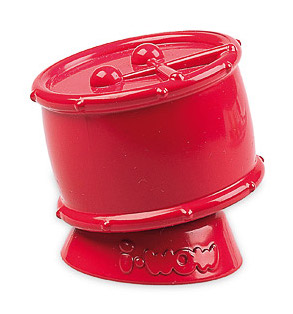
\includegraphics[width=100pt]{graphics/architecture/pieces/piecePercussion.jpg}
	\vspace{0.6cm}
	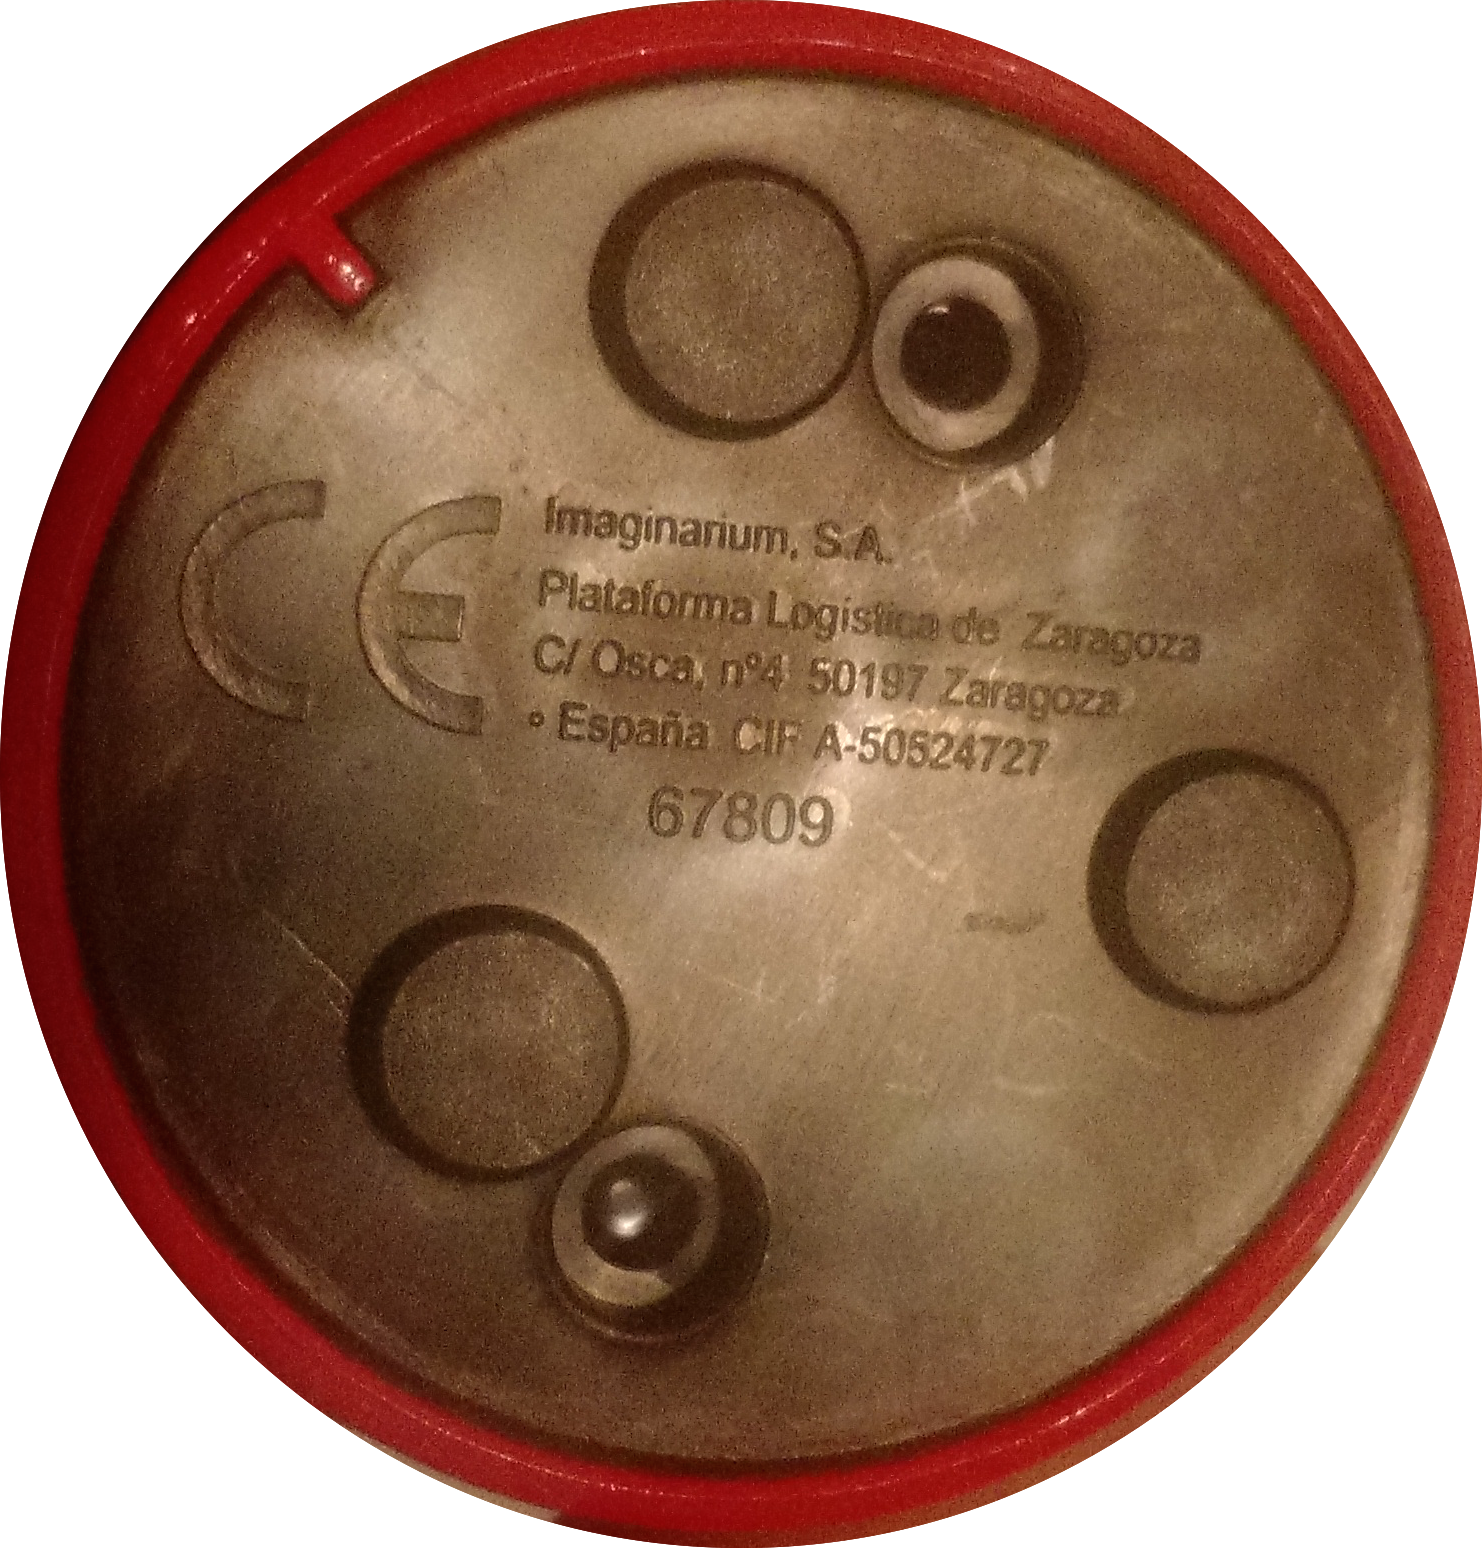
\includegraphics[width=100pt]{graphics/architecture/pieces/percussionBase.png}
	\caption{Drum piece (frontal and base)}
	\label{fig:percussionpiece}
\end{figure}

\begin{figure}[ht!]
	\centering
	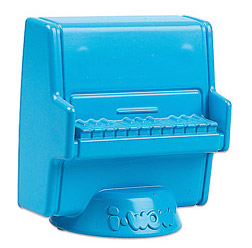
\includegraphics[width=100pt]{graphics/architecture/pieces/pieceKeyboards.jpg}
	\vspace{0.6cm}
	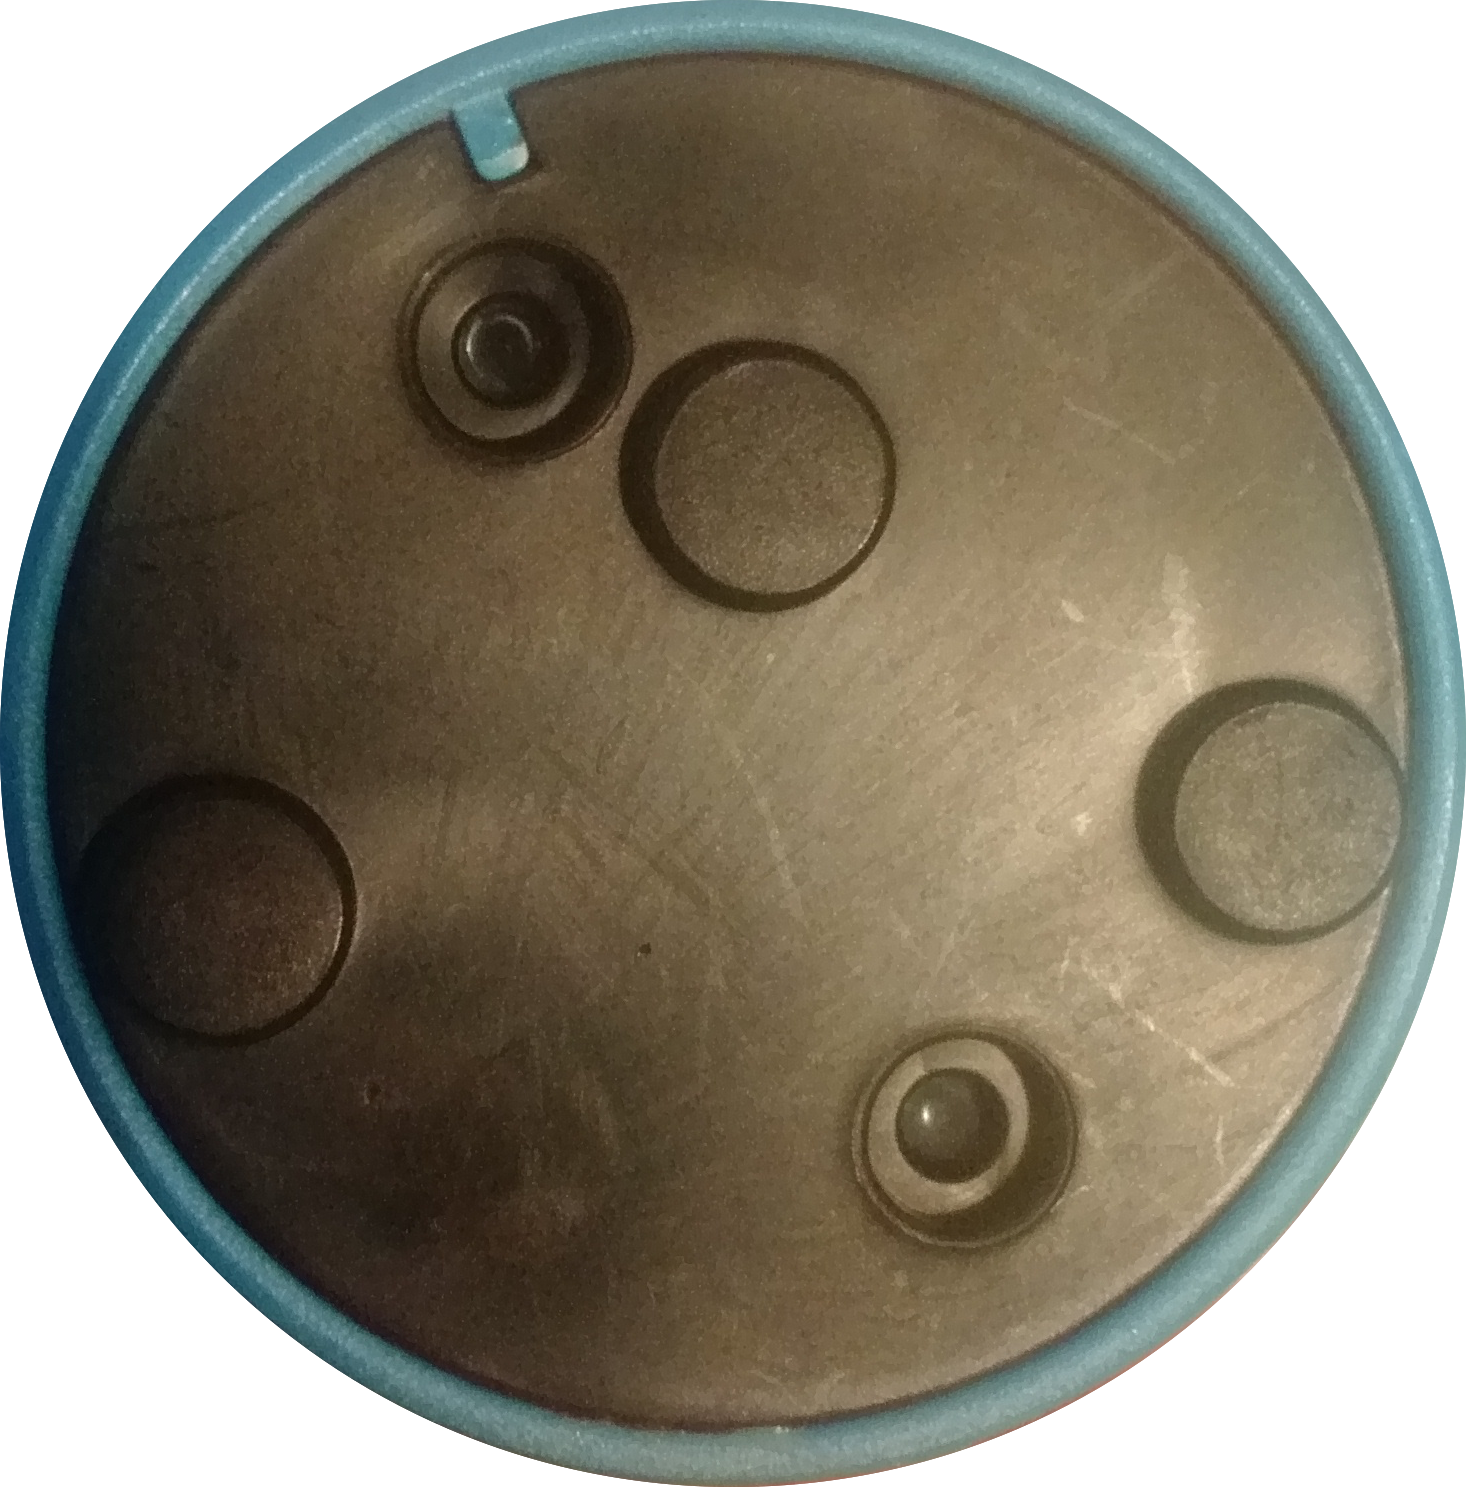
\includegraphics[width=100pt]{graphics/architecture/pieces/keyboardsBase.png}
	\caption{Piano piece (frontal and base)}
	\label{fig:keyboardspiece}
\end{figure}

\begin{figure}[ht!]
	\centering
	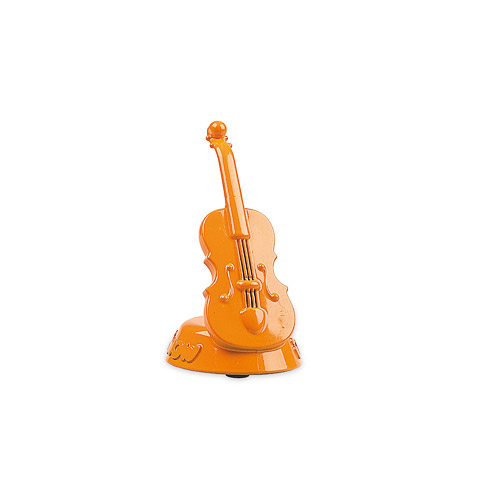
\includegraphics[width=100pt]{graphics/architecture/pieces/pieceStrings.jpg}
	\vspace{0.6cm}
	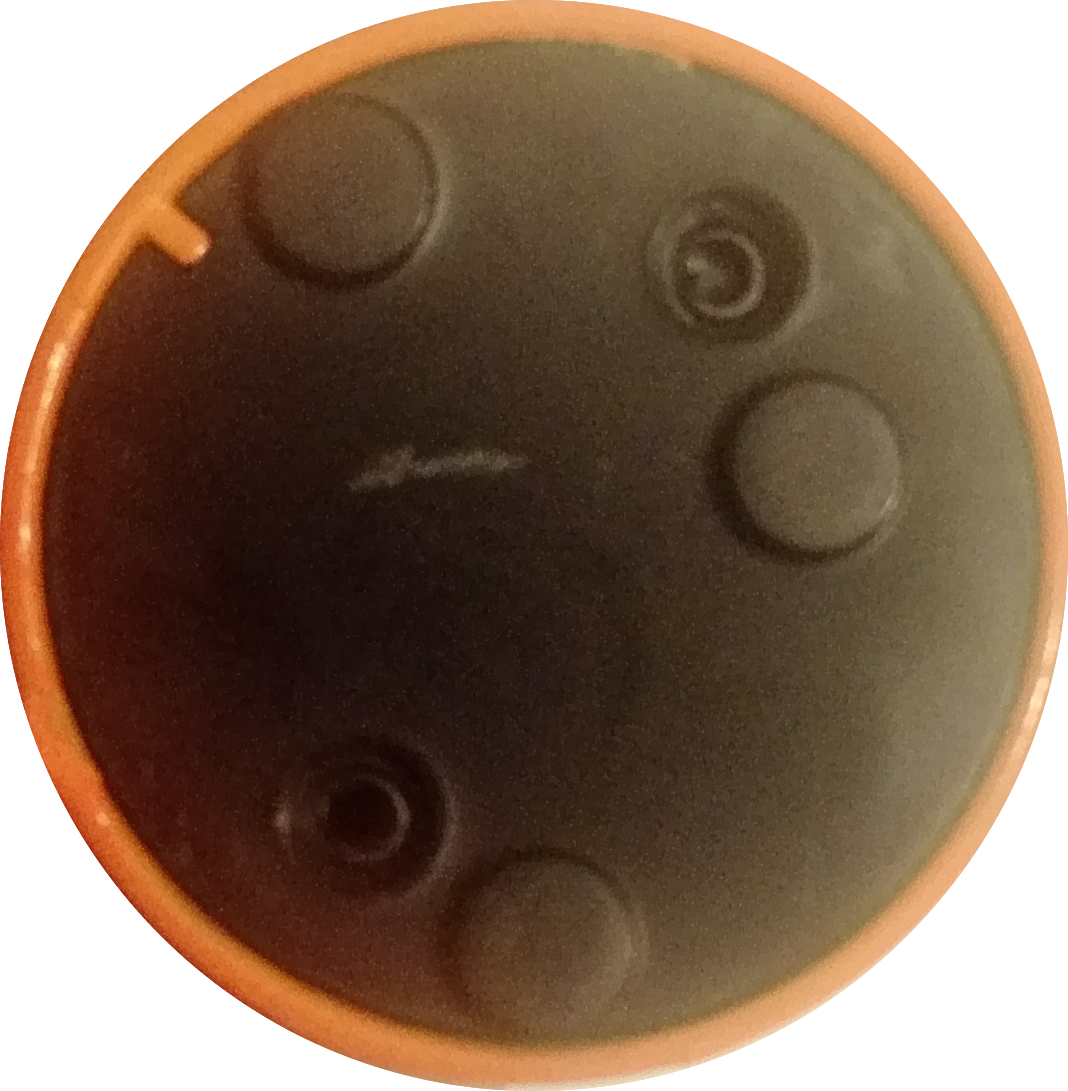
\includegraphics[width=100pt]{graphics/architecture/pieces/stringsBase.png}
	\caption{Violin piece (frontal and base)}
	\label{fig:stringspiece}
\end{figure}

\begin{figure}[ht!]
	\centering
	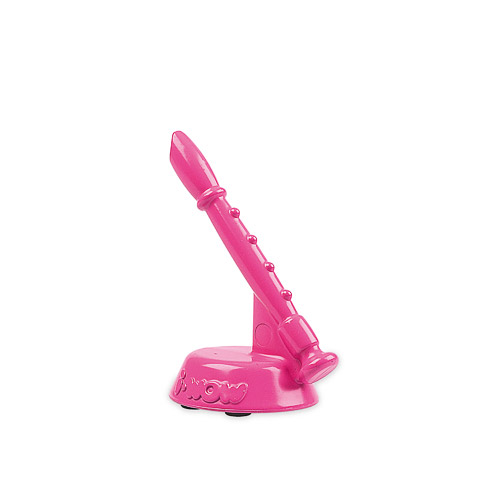
\includegraphics[width=100pt]{graphics/architecture/pieces/pieceWoodwind.jpg}
	\vspace{0.6cm}
	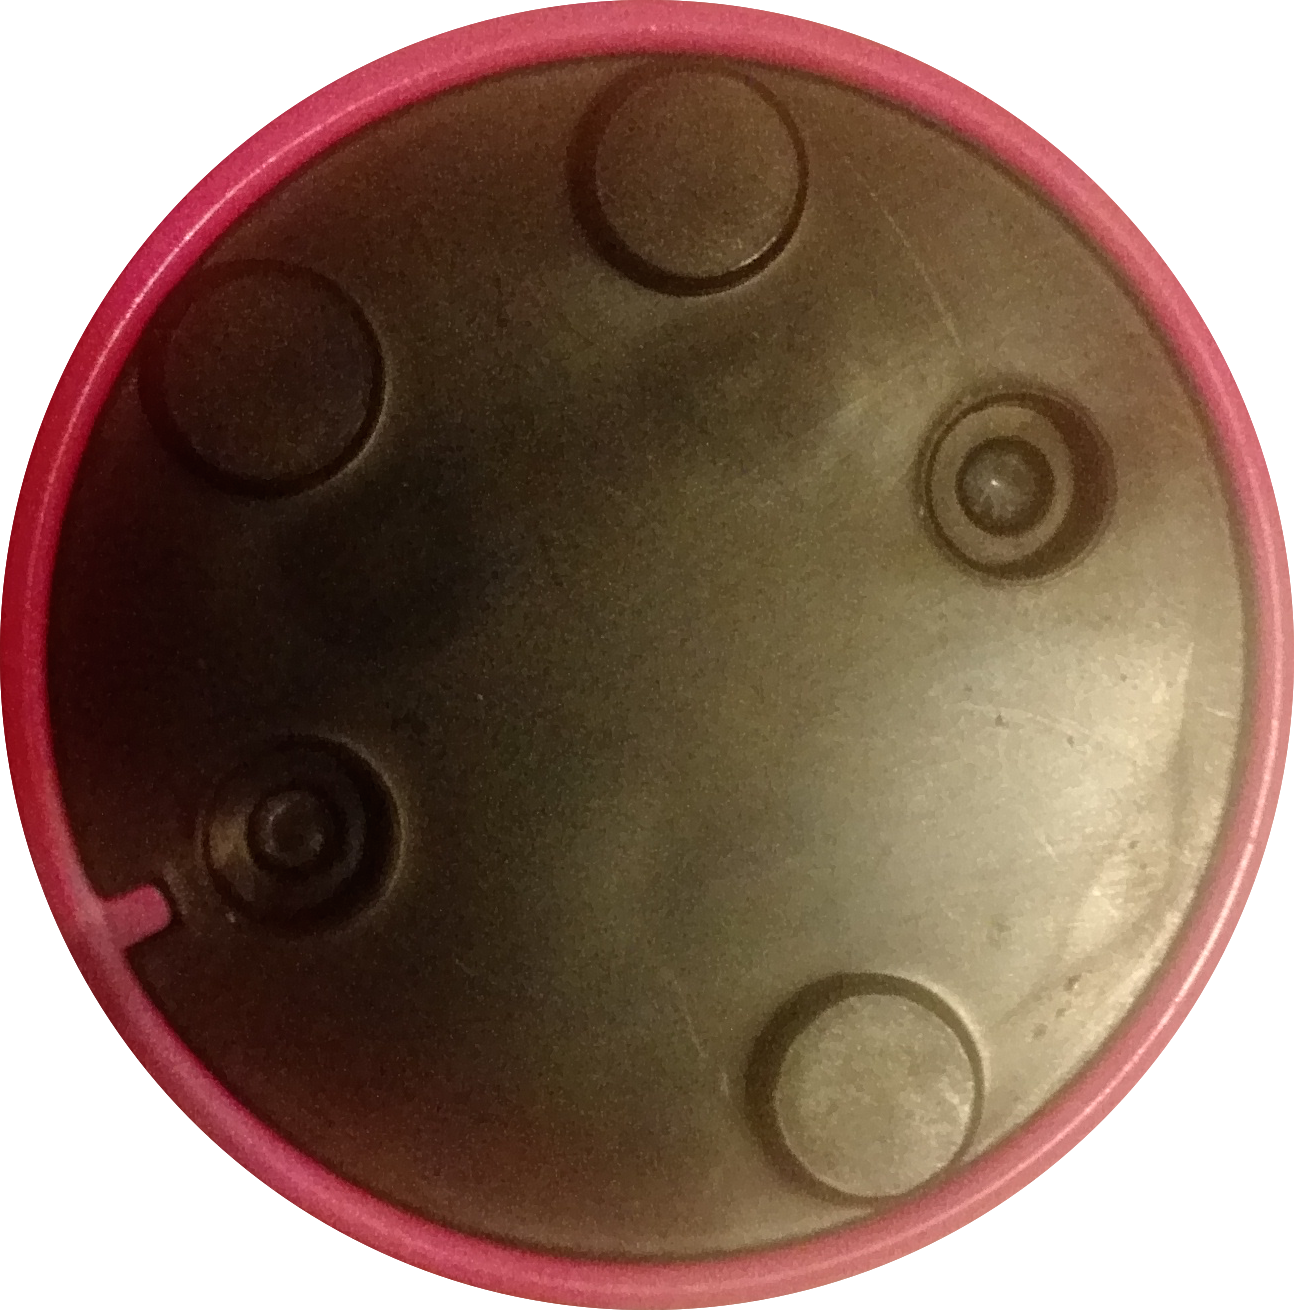
\includegraphics[width=100pt]{graphics/architecture/pieces/woodwindBase.png}
	\caption{Flute piece (frontal and base)}
	\label{fig:woodwindpiece}
\end{figure}

\begin{figure}[ht!]
	\centering
	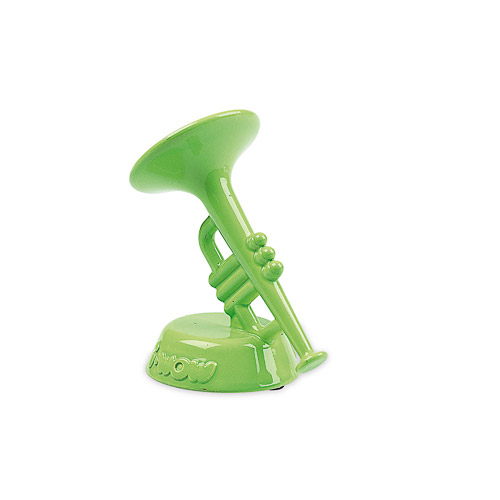
\includegraphics[width=100pt]{graphics/architecture/pieces/pieceBrass.jpg}
	\vspace{0.6cm}
	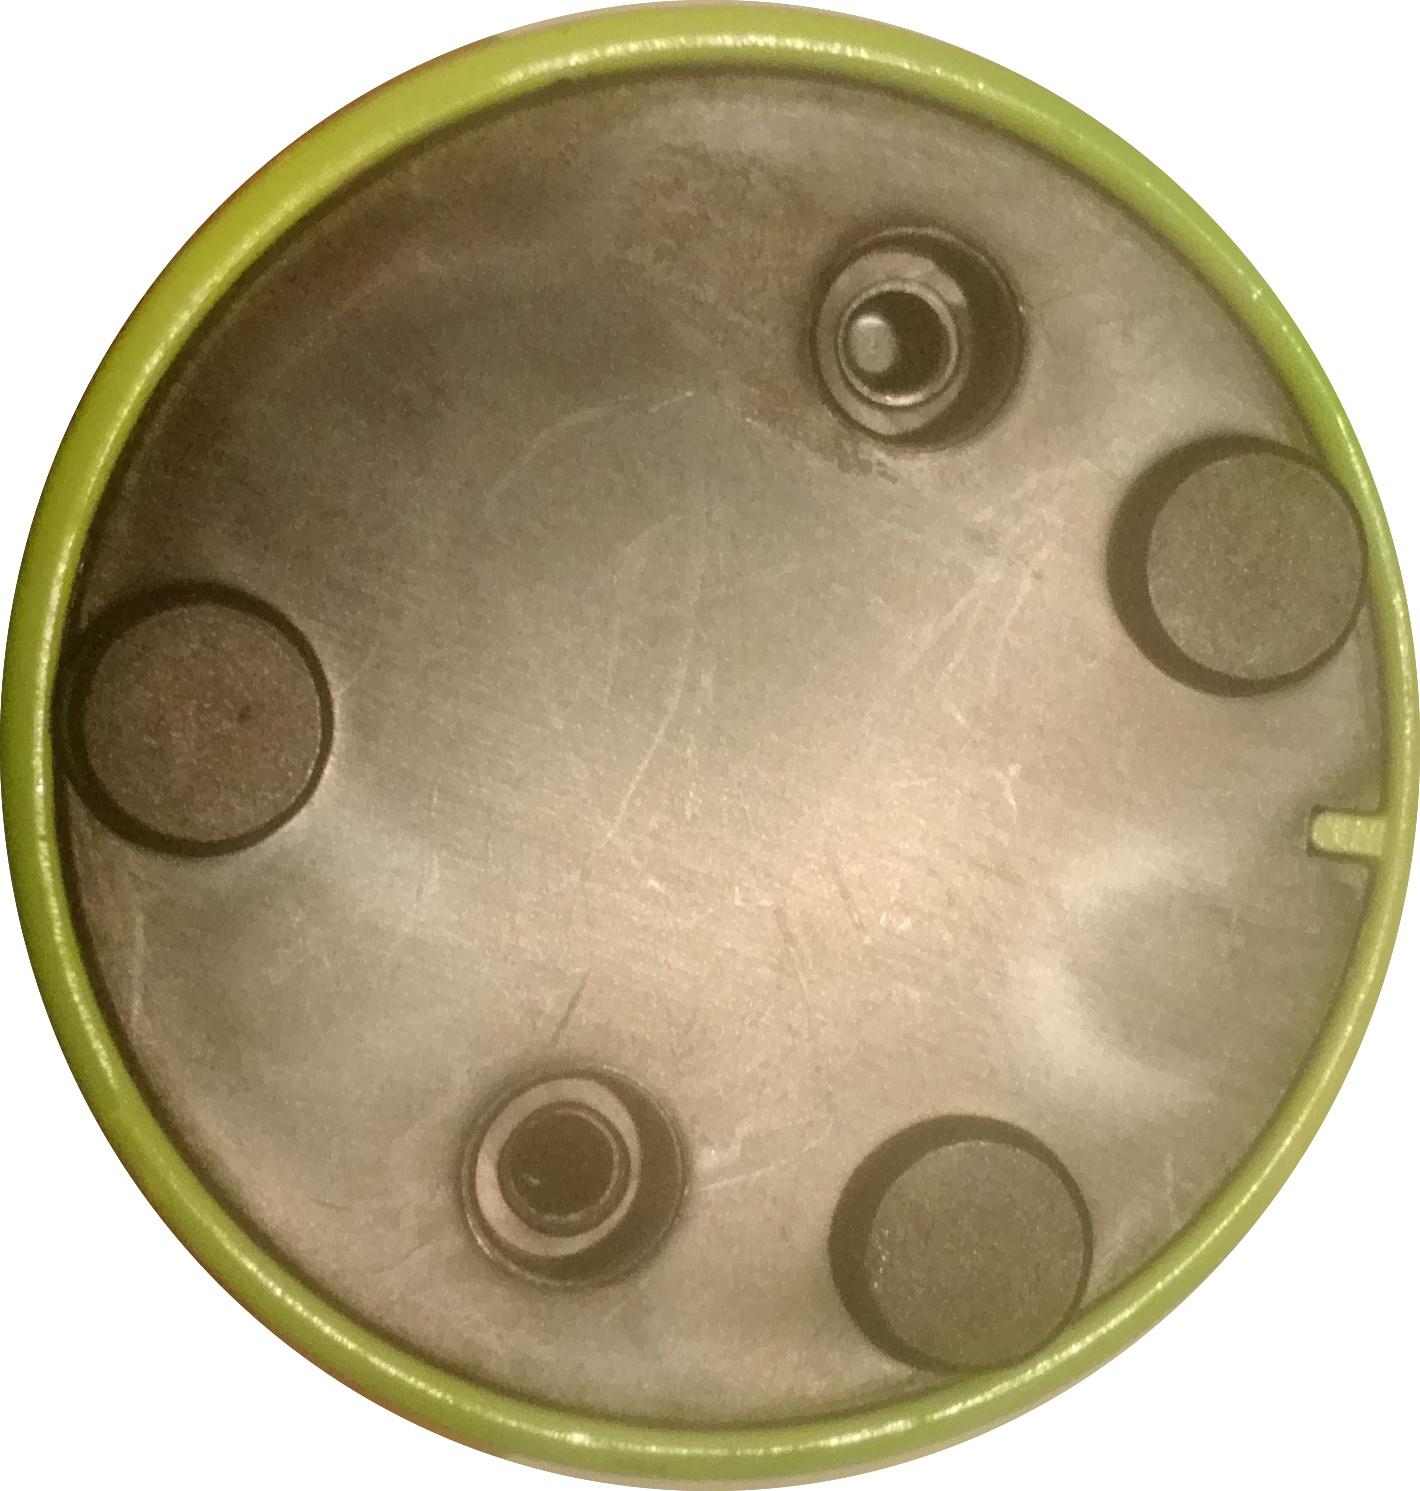
\includegraphics[width=100pt]{graphics/architecture/pieces/brassBase.png}
	\caption{Trumpet piece (frontal and base)}
	\label{fig:brasspiece}
\end{figure}
\FloatBarrier

As we see in the figures above, each figure base has three little pads. These pads are used in order to determine which piece has the gamer placed on the screen. Each piece has their pads placed in a certain position. A more detailed version of the piece bases are shown below:

\begin{figure}[ht!]
	\centering
	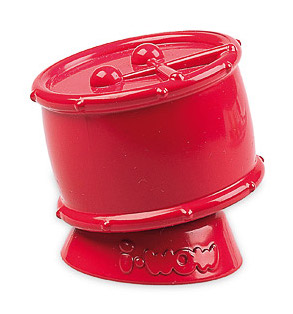
\includegraphics[width=100pt]{graphics/architecture/pieces/piecePercussion.jpg}
	\vspace{0.6cm}
	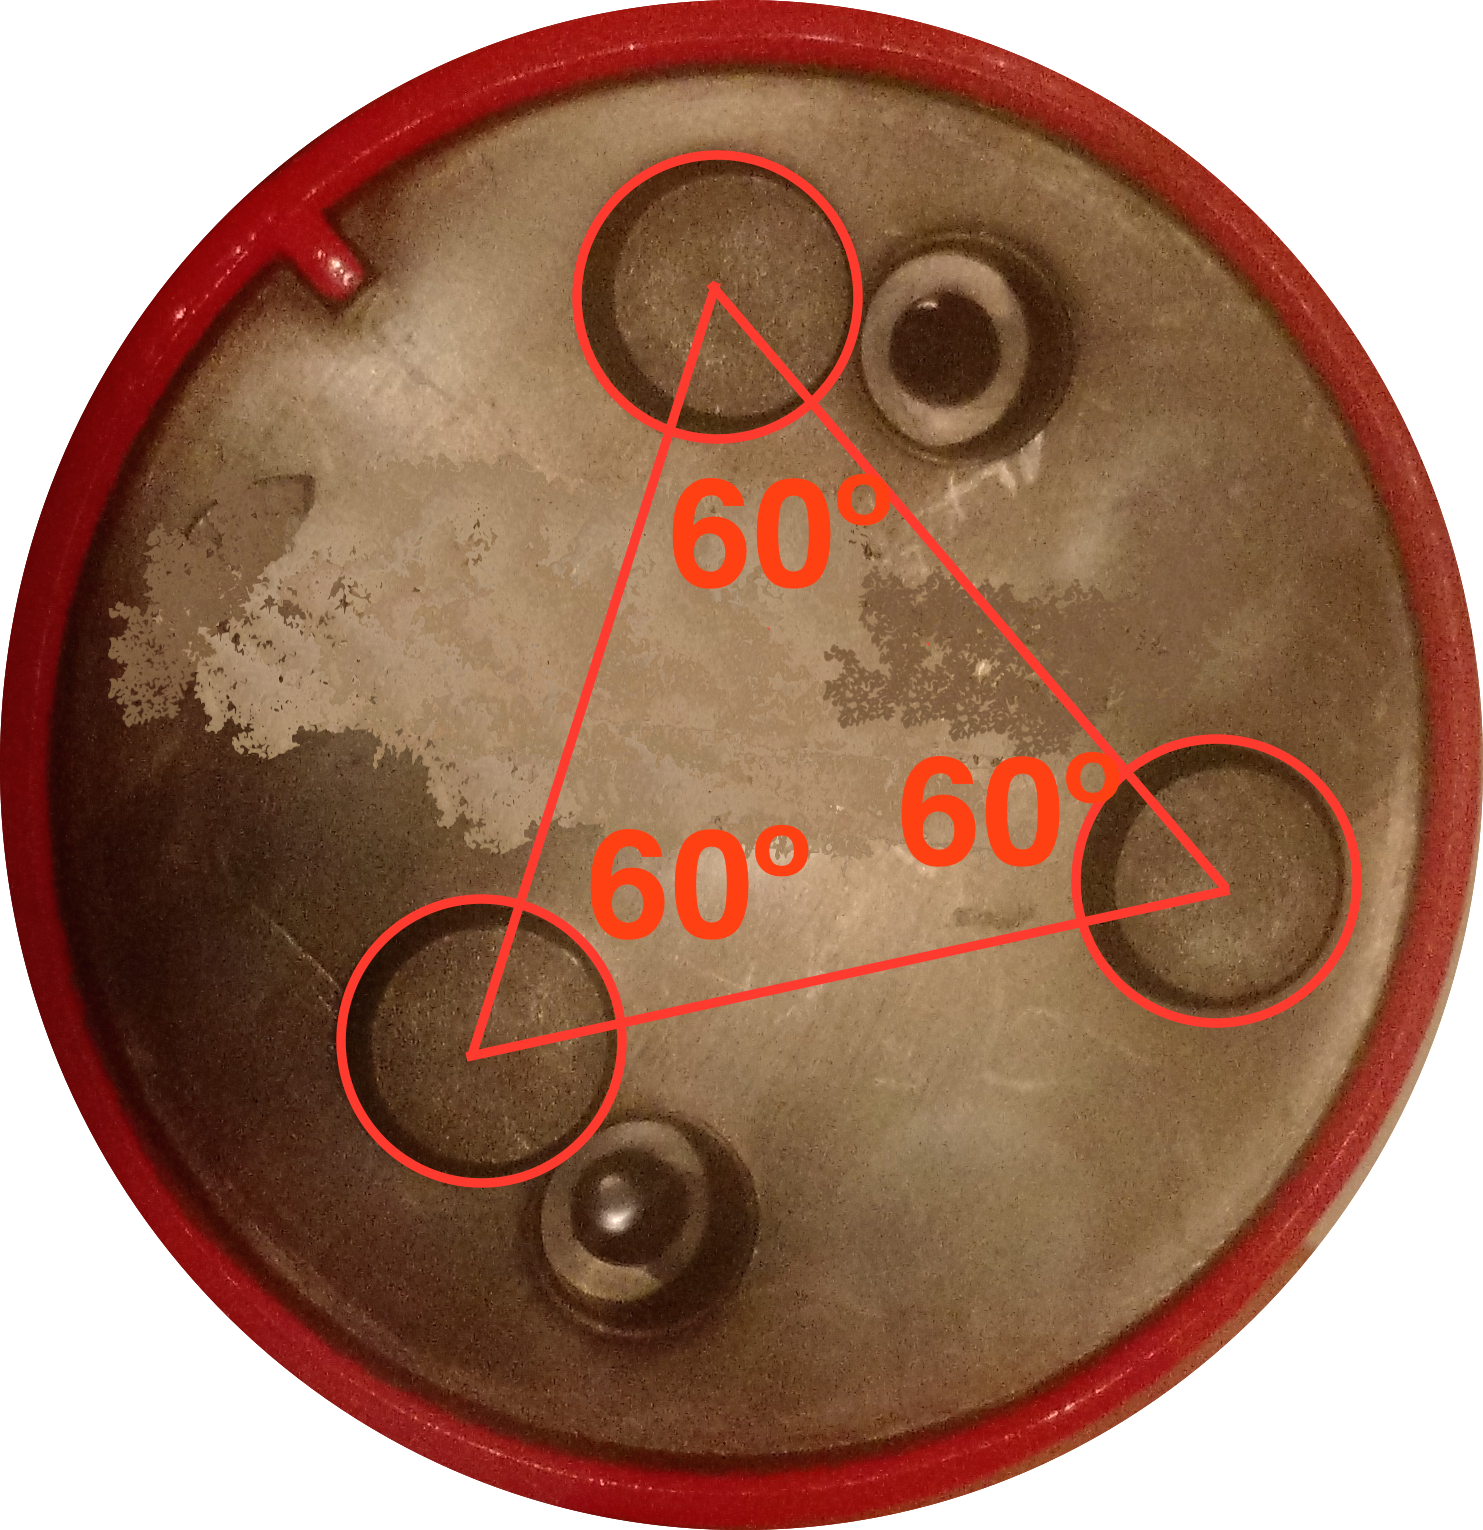
\includegraphics[width=100pt]{graphics/architecture/pieces/percussionBaseAngles.png}
	\caption{Detail of the drum base}
	\label{fig:percussionpiecedetailed}
\end{figure}

\begin{figure}[ht!]
	\centering
	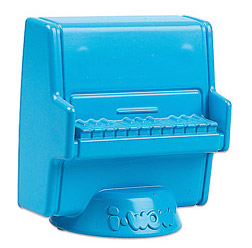
\includegraphics[width=100pt]{graphics/architecture/pieces/pieceKeyboards.jpg}
	\vspace{0.6cm}
	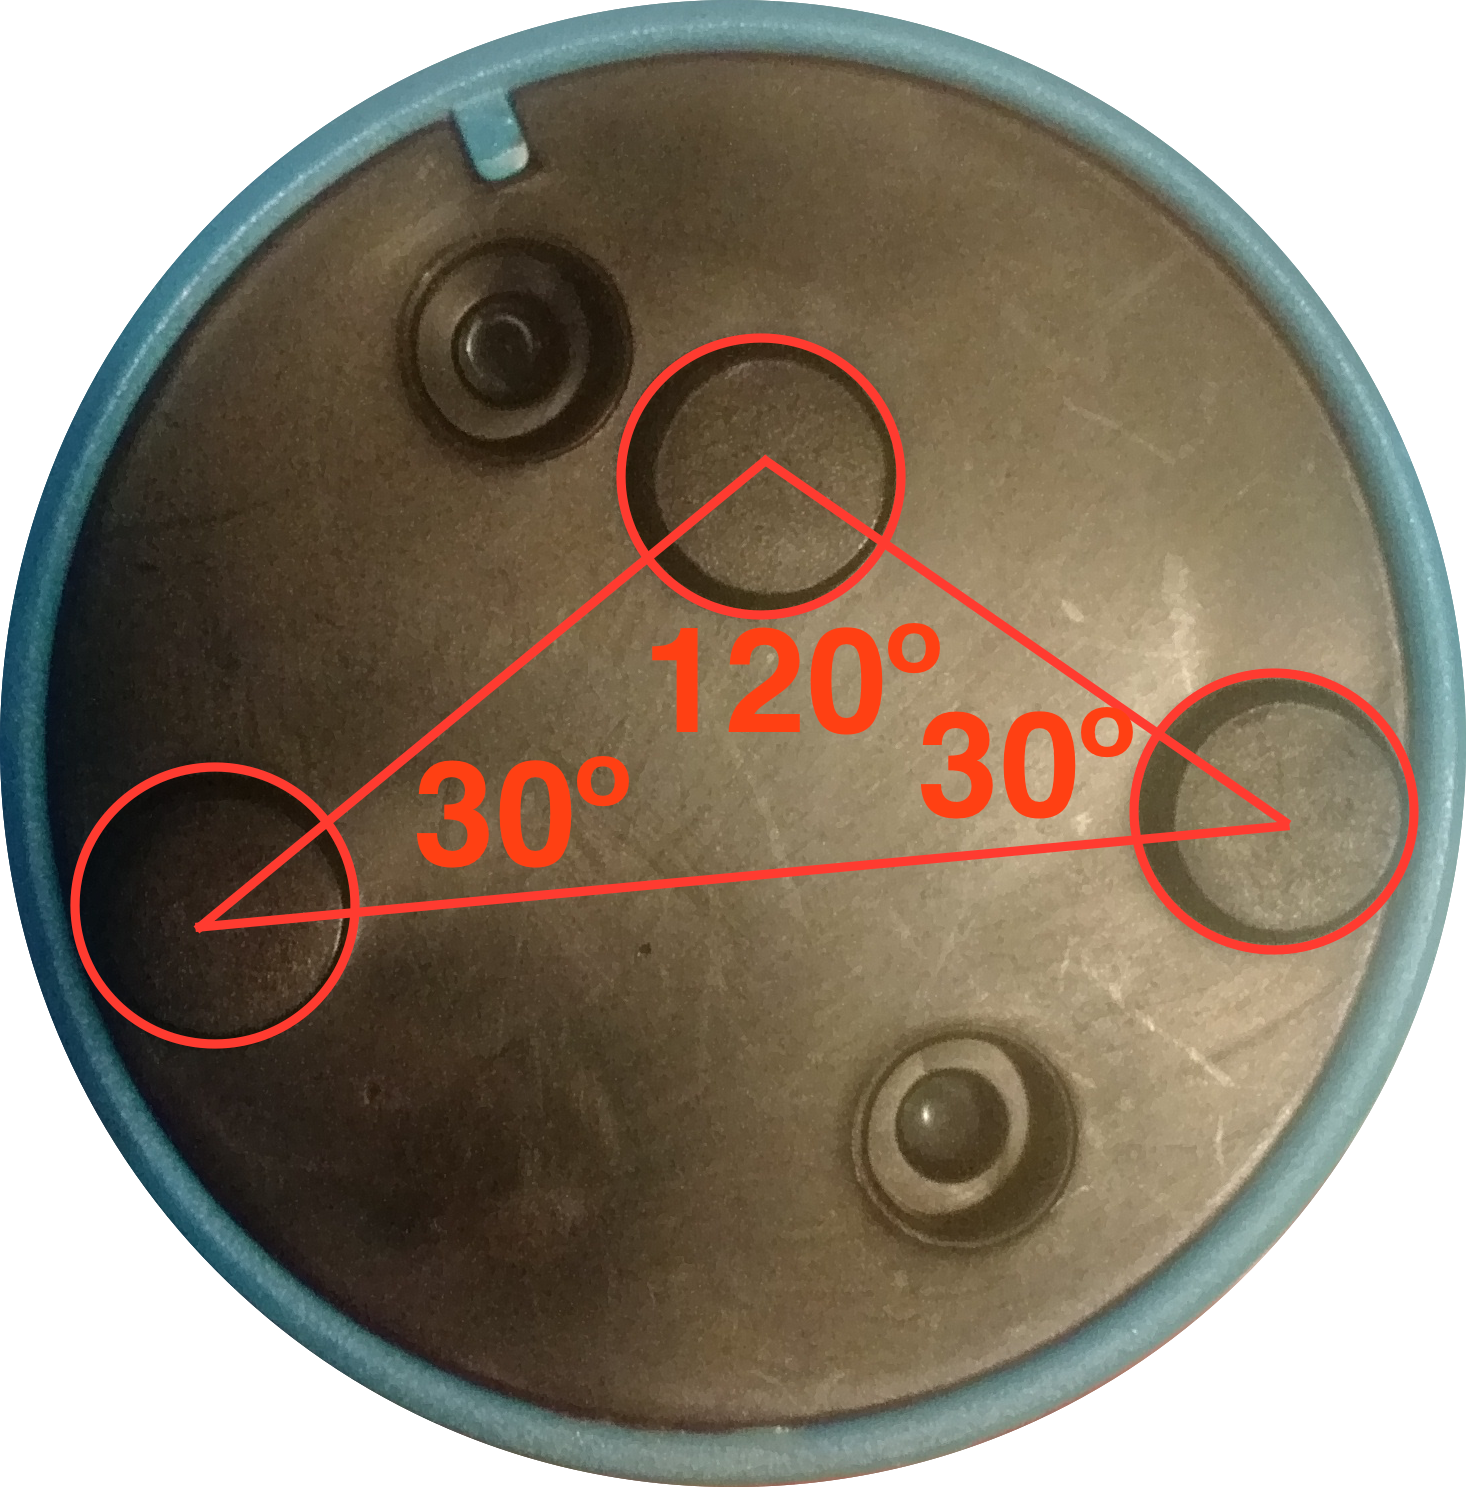
\includegraphics[width=100pt]{graphics/architecture/pieces/keyboardsBaseAngles.png}
	\caption{Detail of the piano base}
	\label{fig:keyboardspiecedetailed}
\end{figure}

\begin{figure}[ht!]
	\centering
	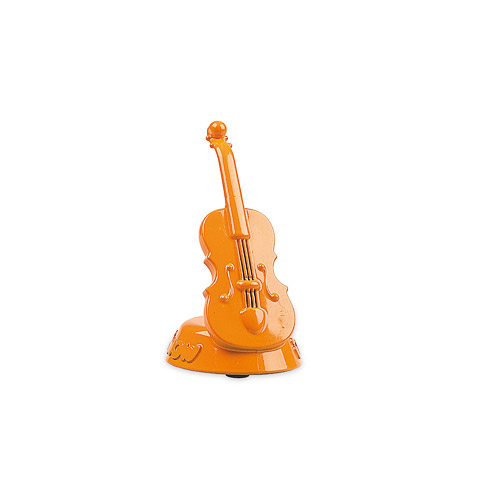
\includegraphics[width=100pt]{graphics/architecture/pieces/pieceStrings.jpg}
	\vspace{0.6cm}
	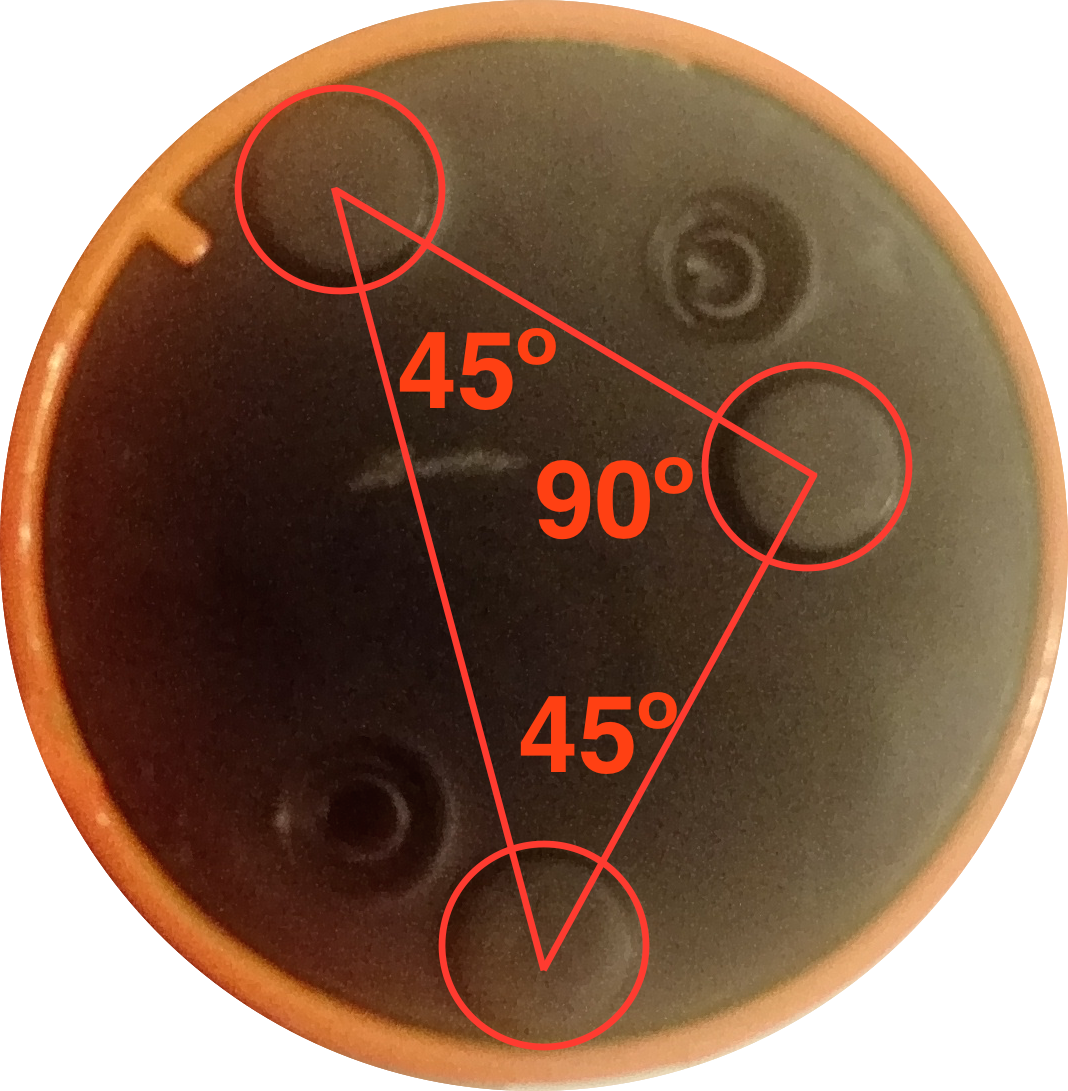
\includegraphics[width=100pt]{graphics/architecture/pieces/stringsBaseAngles.png}
	\caption{Detail of the violin base}
	\label{fig:stringspiecedetailed}
\end{figure}

\begin{figure}[ht!]
	\centering
	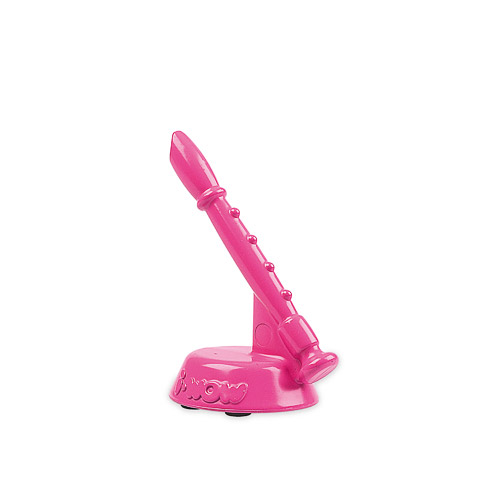
\includegraphics[width=100pt]{graphics/architecture/pieces/pieceWoodwind.jpg}
	\vspace{0.6cm}
	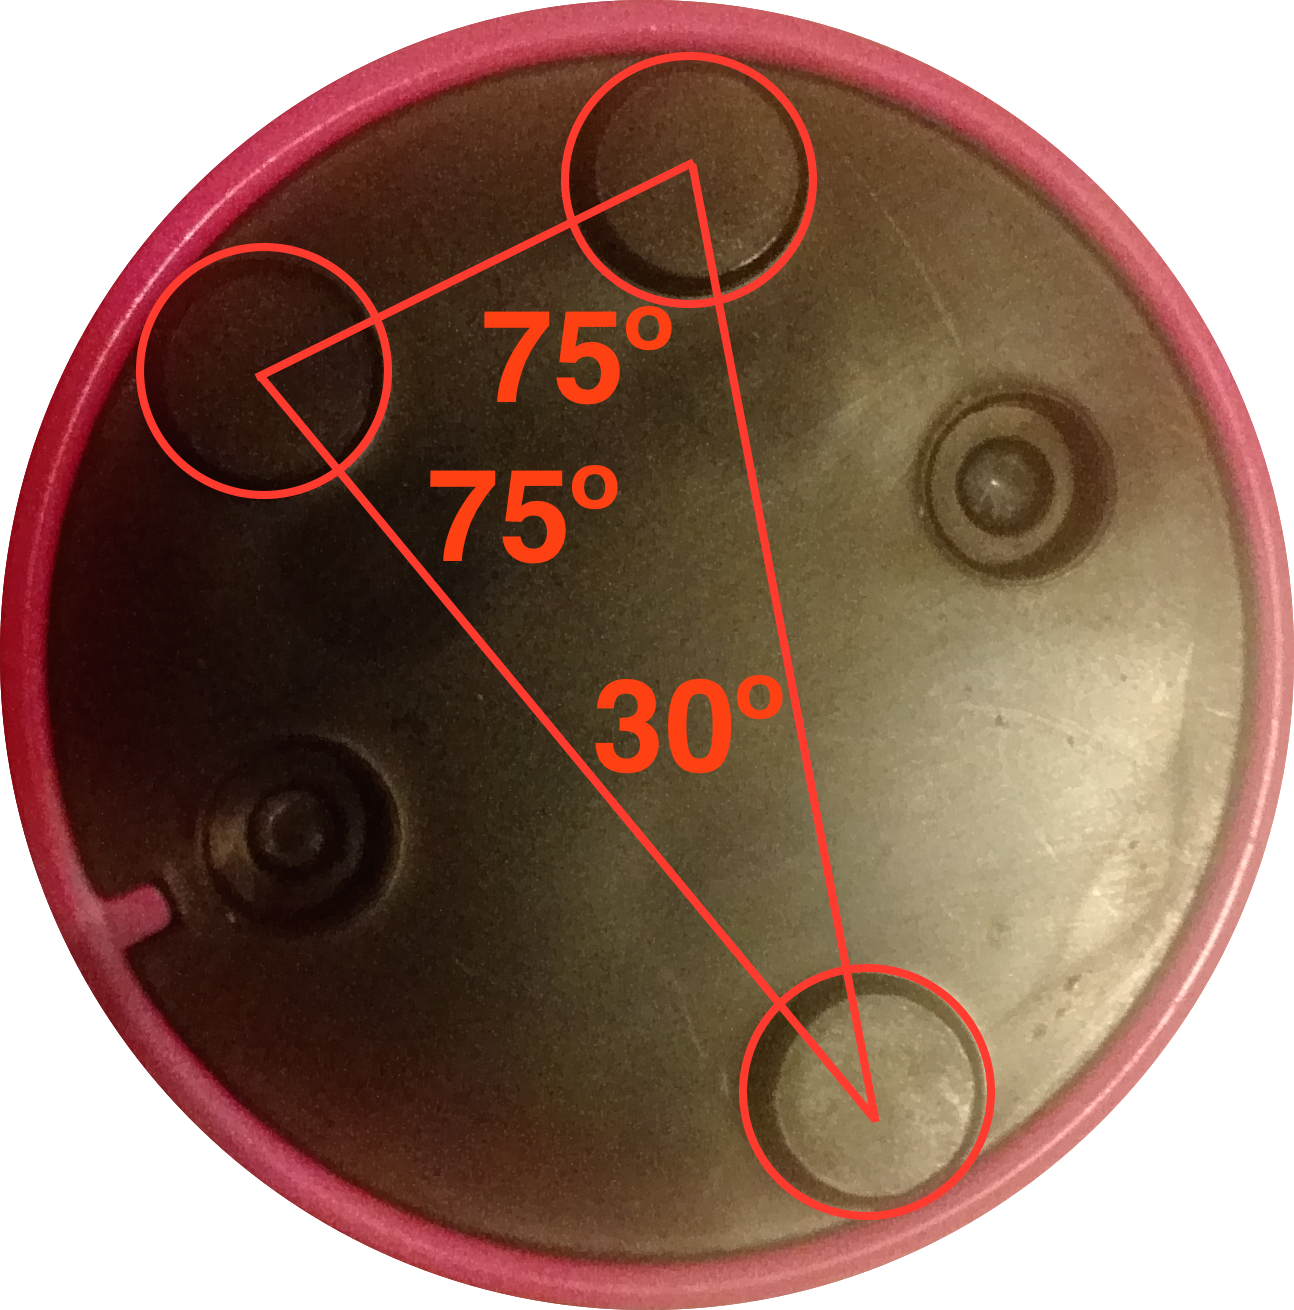
\includegraphics[width=100pt]{graphics/architecture/pieces/woodwindBaseAngles.png}
	\caption{Detail of the flute base}
	\label{fig:woodwindpiecedetailed}
\end{figure}

\begin{figure}[ht!]
	\centering
	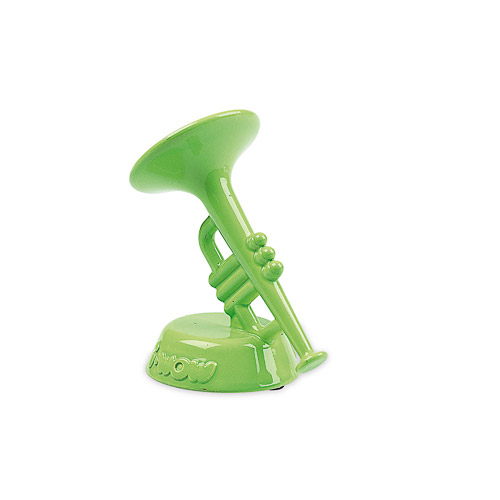
\includegraphics[width=100pt]{graphics/architecture/pieces/pieceBrass.jpg}
	\vspace{0.6cm}
	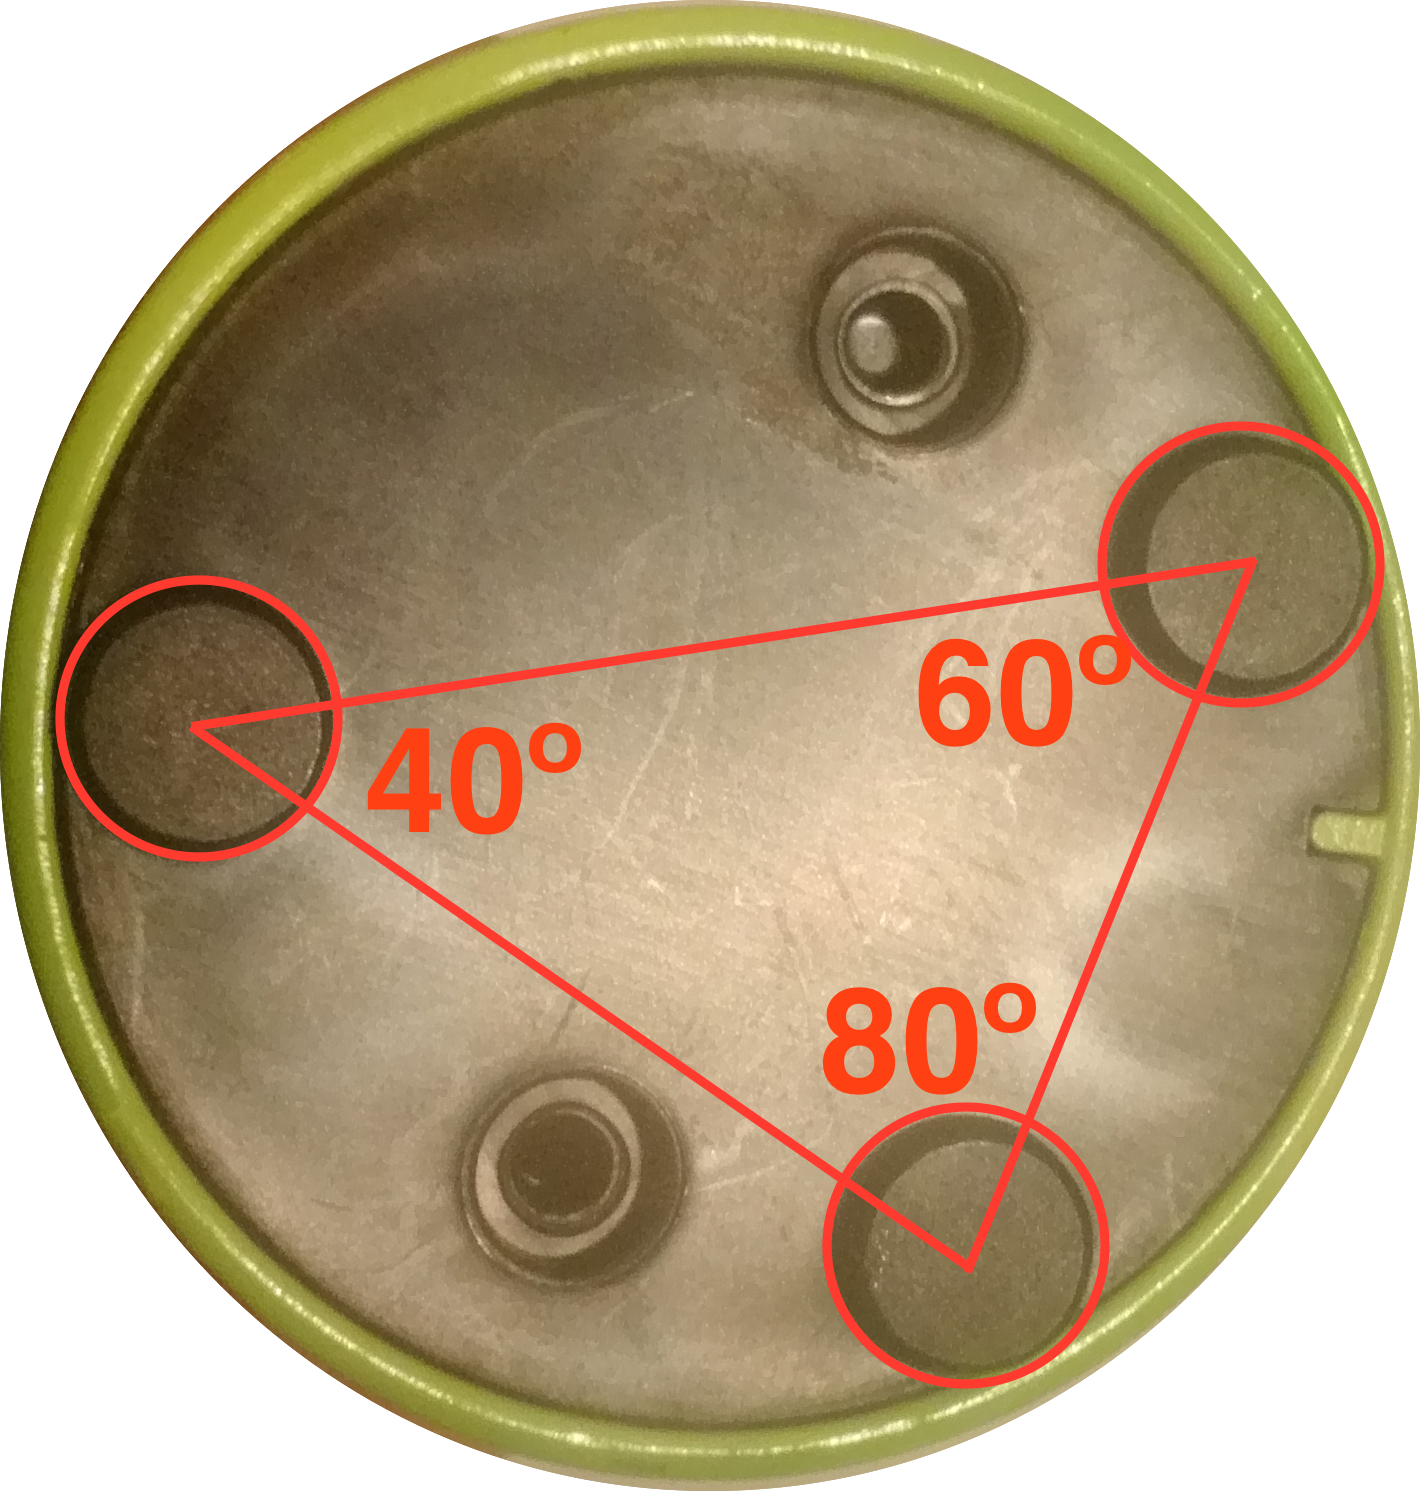
\includegraphics[width=100pt]{graphics/architecture/pieces/brassBaseAngles.png}
	\caption{Detail of the trumpet base}
	\label{fig:brasspiecedetailed}
\end{figure}

\FloatBarrier

As we can see in the above figures, the three pads located in the pieces bases create a triangle. Each piece creates a different triangle with the following angles:
\begin{itemize}
\item \textit{Drum base}, whose triangle has three 60\textdegree\xspace angles, shown in Figure \ref{fig:percussionpiecedetailed}.
\item \textit{Piano base}, whose triangle has two 30\textdegree\xspace angles and one 120\textdegree\xspace angle and two 30\textdegree\xspace angles, shown in Figure \ref{fig:keyboardspiecedetailed}.
\item \textit{Violin base}, whose triangle has two 45\textdegree\xspace angles and one 90\textdegree\xspace angle, shown in Figure \ref{fig:stringspiecedetailed}.
\item \textit{Flute base}, whose triangle has one 30\textdegree\xspace angle and two 75\textdegree\xspace angles, shown in Figure \ref{fig:woodwindpiecedetailed}.
\item \textit{Trumpet base}, whose triangle has one 40\textdegree\xspace angle, one 60\textdegree\xspace angle and one 80\textdegree\xspace angle, shown in Figure \ref{fig:brasspiecedetailed}.
\end{itemize}

Using these angles information the recognition algorithm will be able to determine the placed piece.

\newpage
\subsection{Recognition algorithm}
\label{sec:recognitionalgorithm}
As we have detailed in the previous section, each piece is defined by the triangles on their base. As we know, each triangle is defined by their three angles.

In order to determine the placed piece, we have to retrieve the three intrument pads positions after the gamer places the piece on the recogtion zone. This information will be the input of the algorithm that we have developed to determine the placed musical instrument.

We can see the recognition algorithm in Figure \ref{fig:detectionalgorithm}.

\begin{figure}[ht!]
	\centering
	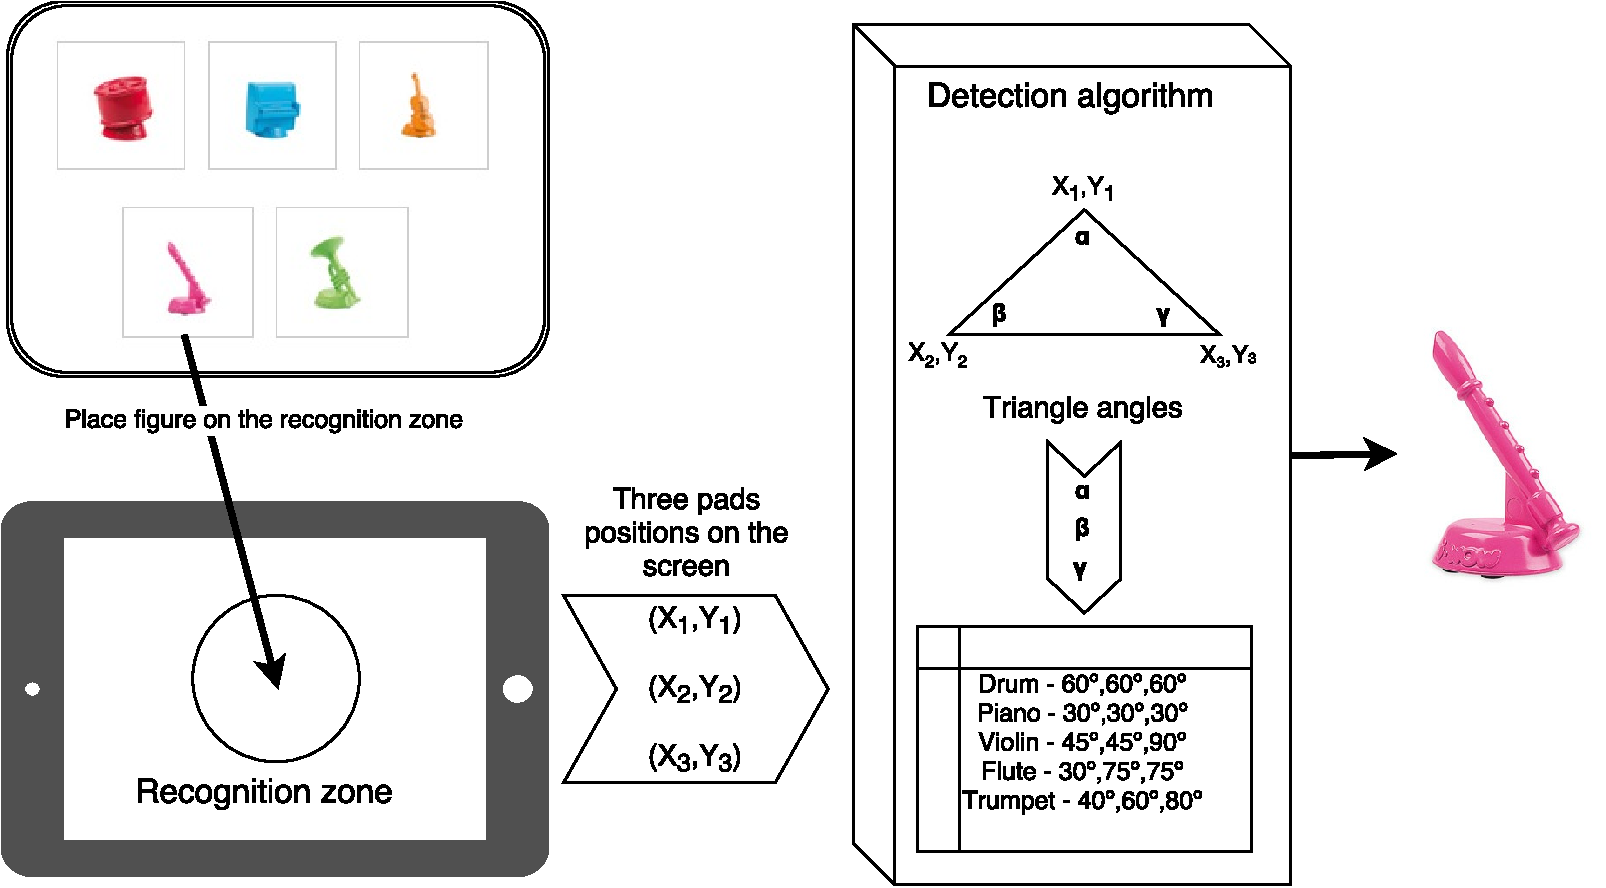
\includegraphics[width=400pt]{graphics/architecture/DetectionAlgorithm.pdf}
	\caption{Detection algorithm diagram}
	\label{fig:detectionalgorithm}
\end{figure}

If we look at \ref{fig:detectionalgorithm}, we can see how the piece if recognized by the application. This recognition could be divided within three steps:

\begin{enumerate}
	\item The gamer has to place the piece on the recognition zone. When the three pads located in the piece base touch the screen, these pads coordinates $\Bigl(\begin{smallmatrix} x_1&y_1 \\ x_2&y_2 \\ x_3&y_3 \end{smallmatrix} \Bigr)$ are sent to the detection algorithm.
	\item The detection algorithm calculate the angles of a triangle build using the three coordinates given by the piece base.
	\item The detection algorithm compare the calculated triangle with the figure's defined triangles. After it, we retrieve the piece whose base triangle match the calculated one.
\end{enumerate}

We can see the algorithm design below:

\begin{algorithm}[ht!]
 \SetKwData{Left}{left}\SetKwData{This}{this}\SetKwData{Up}{up}
 \SetKwFunction{Union}{Union}\SetKwFunction{FindCompress}{FindCompress}
 \SetKwInOut{Input}{input}\SetKwInOut{Output}{output}

 \Input{$(X_i,Y_i)$ $\forall$ i = 1,2,3 where $X,Y \in \mathbb{R}_2$}
 \Output{Instrument recognized $\in$ \{Drum,Piano,Violin,Flute,Trumpet\}}
 \BlankLine
 initialization\;
 \While{piece is placed on the recognition zone}{
  read current\;
  \eIf{understand}{
   go to next section\;
   current section becomes this one\;
   }{
   go back to the beginning of current section\;
  }
 }
 \caption{Instrument recognition algorithm}
\end{algorithm}

\newpage
\section{Application}
\label{sec:application}
The application is the biggest module of the game. It includes the whole software development as it is shown in Figure \ref{fig:applicationarchitecture}.

\begin{figure}[ht!]
	\centering
	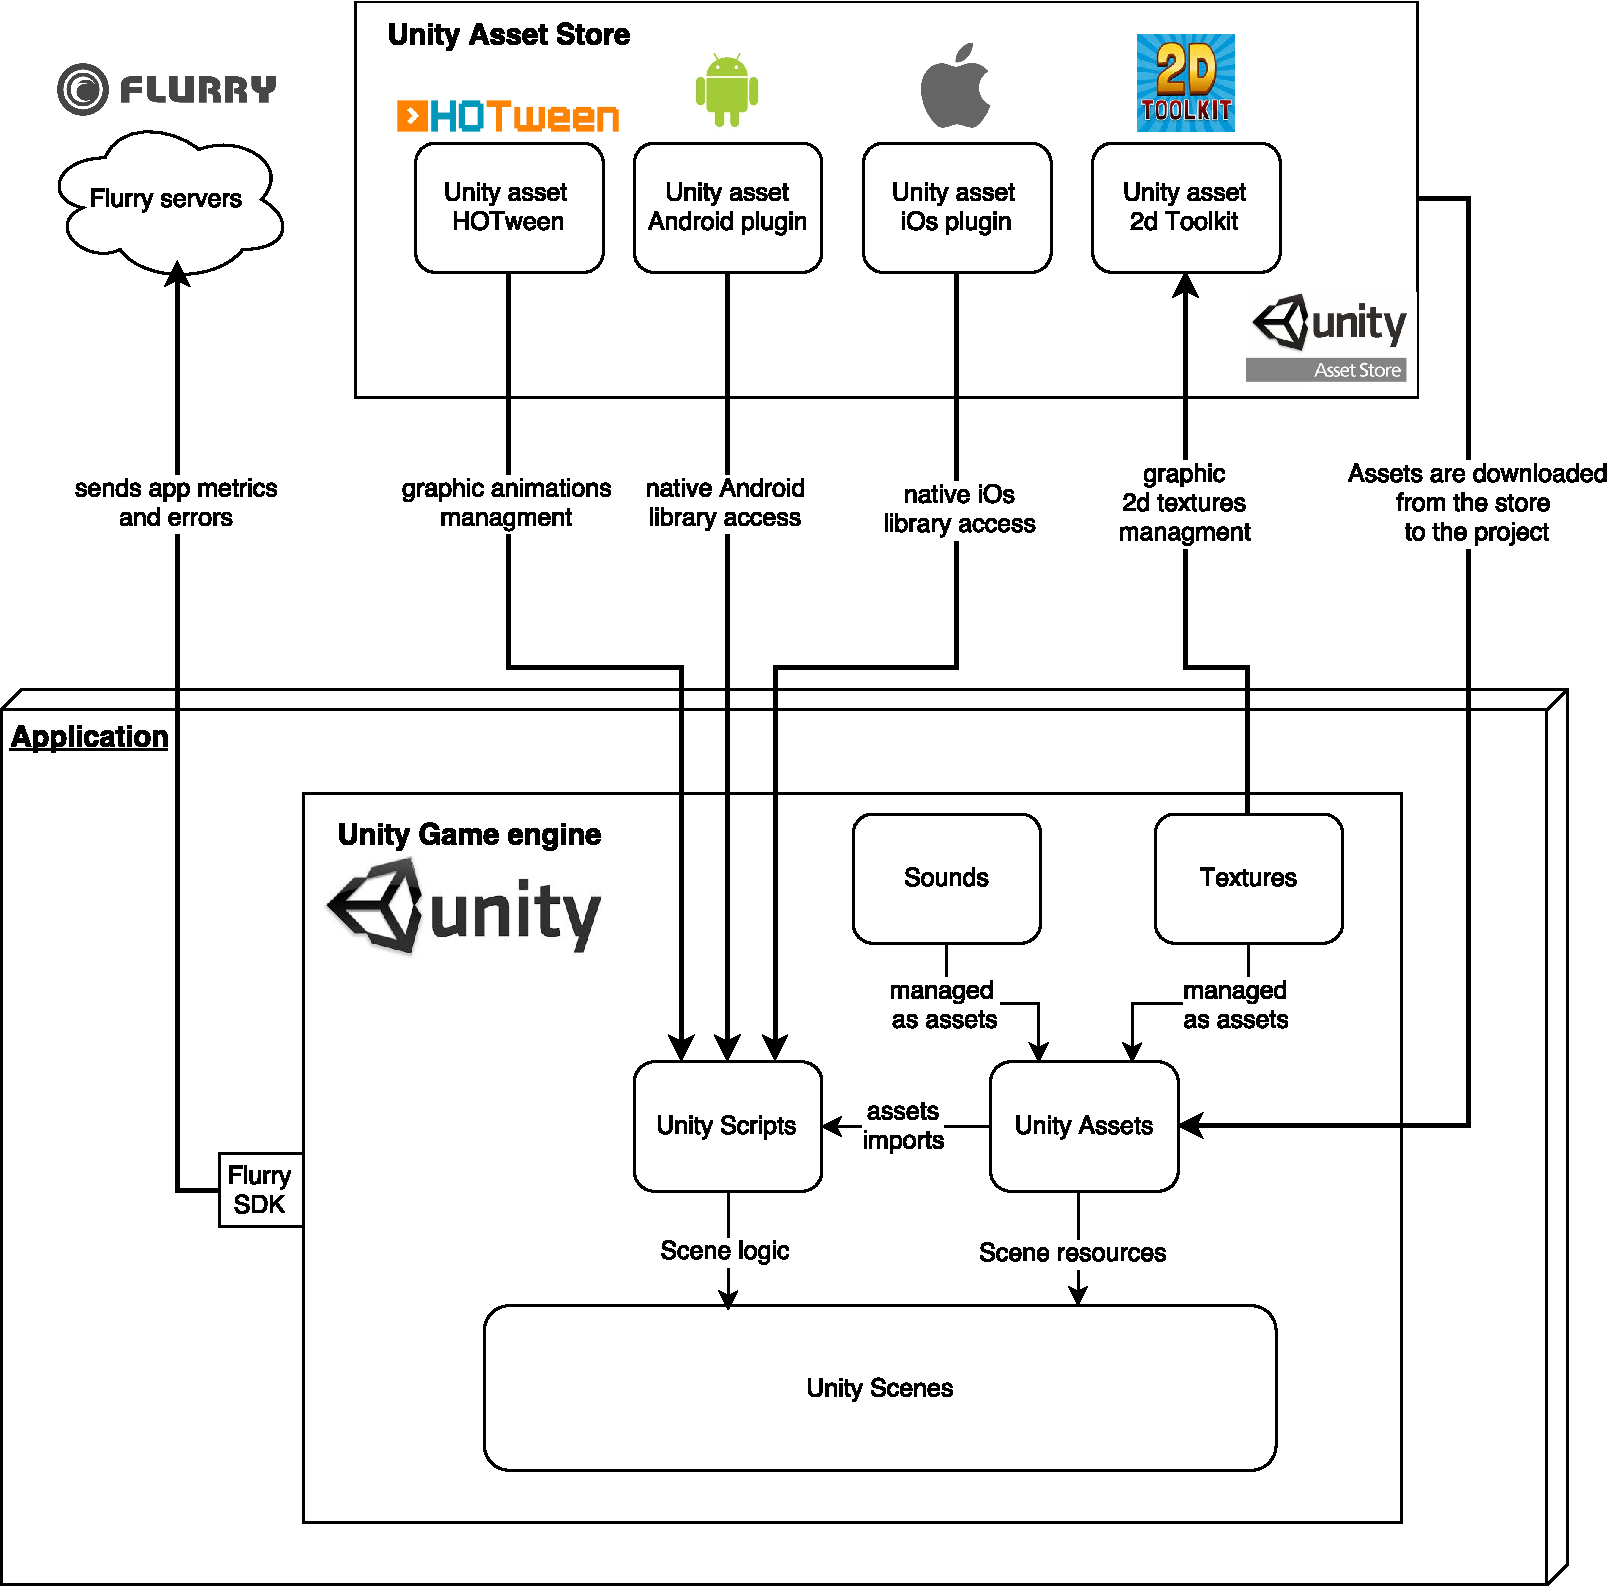
\includegraphics[width=400pt]{graphics/architecture/Application_architecture.pdf}
	\caption{Application architecture diagram}
	\label{fig:applicationarchitecture}
\end{figure}

If we look at the application architecture diagram we can see the Application module where Unity game engine will run. Unity has three main components, Unity Assets, Unity Scripts and Unity Scenes. These components and Unity interaction with Flurry are described below:

\subsection{Assets}
An asset is a representation of any item that can be used in your game or project. An asset may come from a file created outside of Unity, such as a 3D model, an audio file, an image, or any of the other types of file that Unity supports. There are also some asset types that can be created within Unity, such as an Animator Controller, an Audio Mixer or a Texture Managers. In other words, assets are any resource your game uses.

Thankfully, Unity’s asset importing is robust and intelligent, it will accept all popular 3D file formats and also supports all common image file formats, including PNG, JPEG, TIFF and even layered PSD files directly from Photoshop. When it comes to audio, Unity supports WAV and AIF, ideal for sound effects, and MP3 and OGG for music.

In Figure \ref{fig:applicationarchitecture} we can see that sounds and textures are included as assets to use them, but they are not the only assets we will use. We said that there are some assets types that have been created within Unity to make development easier. In our case we will use an Animation Controller called HOTween, a 2D Texture Manager called 2dToolkit and both Android and iOs plugins. All these assets are included in our Unity project downloading them from Unity Asset Store.

The Unity Asset Store is where a growing library of free and commercial assets are placed. These assets are created both by Unity Technologies and also members of the community. A wide variety of assets is available, covering everything from textures, models and animations to whole project examples, tutorials and Editor extensions. These assets are accessed from a simple interface built into the Unity Editor and are downloaded and imported directly into your project.

Assets will be used from the Scenes and/or the Scripts, which are detailed in section \ref{subsec:unityscripts}.

\subsection{Scenes}
Scenes contain the objects of your game. They can be used to create a main menu, individual levels, and anything else. Each unique Scene file as a unique level, where you will place your environments, obstacles, and decorations, essentially designing and building your game in pieces.

We can easily make an analogy between Scenes and screens in our app. Each screen is built from a Scene where all the Assets logic are managed by the Scripts.

Creating Scenes with Unity are possible thanks to their intuitive interface, where project assets can be drag to the interface Scene and Scripts can be attached to the assets to control them.

\subsection{Scripts}
\label{subsec:unityscripts}
Scripts, known in Unity as behaviors, let you take assets in your scene and make them interactive. Multiple scripts can be attached to a single object, allowing for easy code reuse. Unity supports three different programming languages; UnityScript, C\#, and Boo. In our project we will use C\#.

As we can see in Figure \ref{fig:applicationarchitecture}, Scripts will manage Unity Assets and will use external Assets from the Unity Asset Store as libraries to make the development easier. In our case, HOTween asset allow us to automate the animation of any numeric (and some non-numeric) property or field (numbers, vectors, transforms, and so on) in many different ways. 2dToolkit provide an efficient 2D sprite, collider set-up and text system which integrates seamlessly into the Unity environment. Android and iOs plugins allow us to access to native Android and iOs libraries.

As we said, scripts will be attached to the scene assets we need to provide them the functionality we need to.

\subsection{Flurry}
Flurry analytics allow us to easily add analytics to our mobile game applications. Integrating this technology within our application will allow us to retrieve game application metrics such as volume of users, time of use or crash reports.

As we can see in Figure \ref{fig:applicationarchitecture}, in order to integrate it into our development we have to add Flurry SDK into our Unity project. Before that we just have to create a project using Flurry web application. After all this process we will be able to use flurry library to manage all the components we want to. In our case we will retrieve the following metrics:

\begin{itemize}
\item \textit{Active users}, the total number of unique users who accessed the application per day.
\item \textit{New users}, the total number of unique users who used the application for the first time per day.
\item \textit{Average session length}, average length of a user session per day.
\item \textit{Crash analytics}, information about the application crashes, exceptions and errors.
\end{itemize}

\section{Application use workflow}
The application has three game modes, for each one we will see the application use workflow to get a more precise idea of how the Gamer will interact with the application.

The three game modes were designed as a result of the Game modes use case defined in section \ref{subsec:gamemodes}:

\begin{itemize}
\item \textit{Playing instrument game mode} detailed in sub-section \ref{subsec:playinstrument_arch}.
\item \textit{Conducting orchestra game mode} detailed in sub-section \ref{subsec:conducteorchestra_arch}.
\item \textit{Discovering instrument game mode}  detailed in sub-section \ref{subsec:discoverinstrument_arch}.
\end{itemize}

\newpage
\subsection{Playing instrument game mode}
\label{subsec:playinstrument_arch}

Playing instrument game mode workflow is represented in Figure \ref{fig:playingworkflow}

\begin{figure}[ht!]
	\centering
	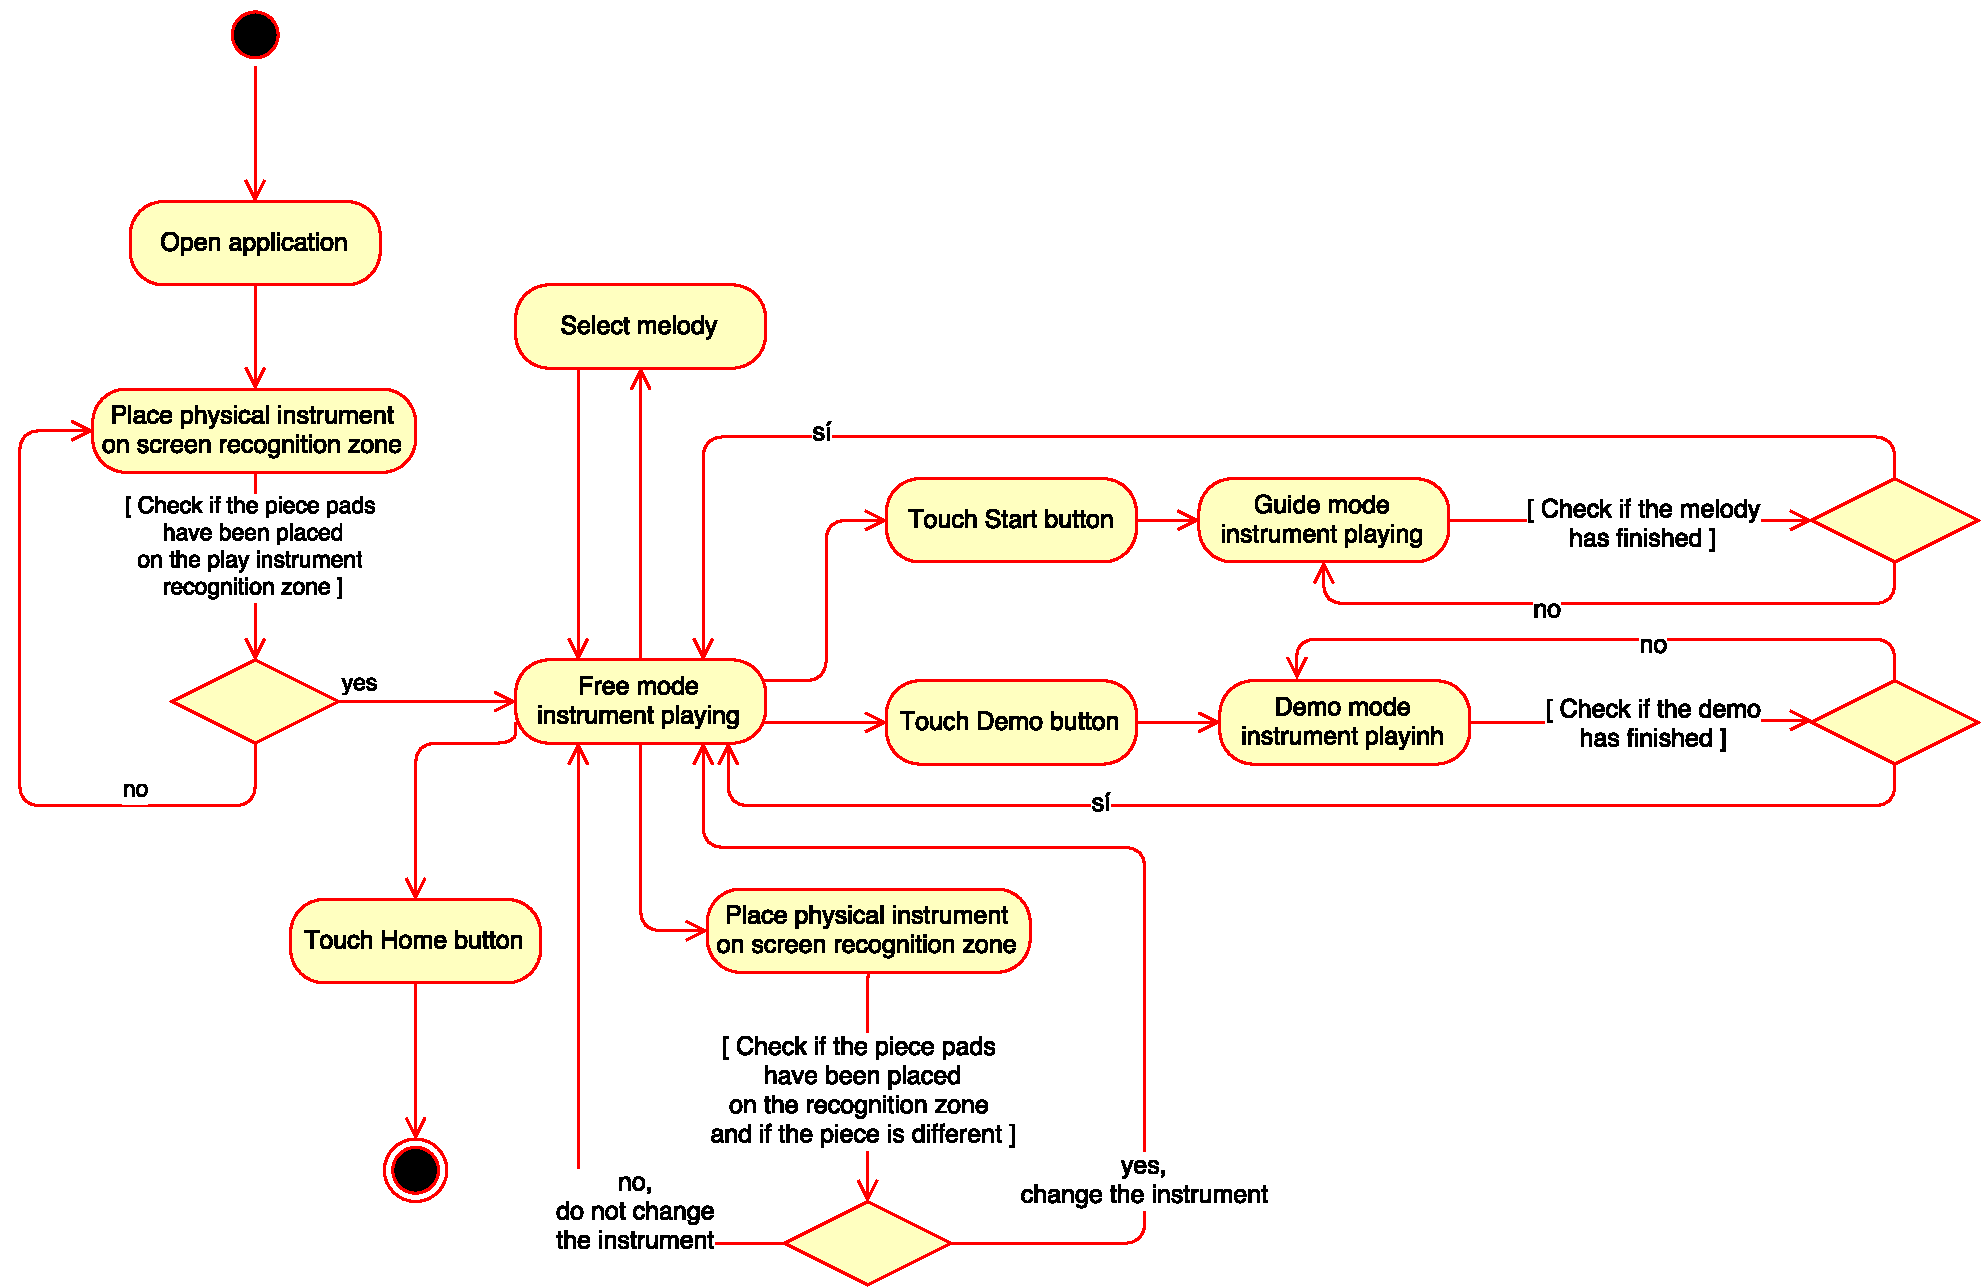
\includegraphics[width=400pt]{graphics/architecture/PlayingGameMode.pdf}
	\caption{Playing instrument game mode}
	\label{fig:playingworkflow}
\end{figure}

As we can see in Figure \ref{fig:playingworkflow}, to access \textit{Playing instrument game mode}, the gamer has to place the physical instrument miniature in the Playing mode recognition zone after opening the application. If the instrument has been placed properly, the \textit{Free mode instrument play} screen is opened.

Within this \textit{Free mode instrument play} screen, the gamer can play freely with the instrument that has been placed to access to this game mode. Also, the gamer is able to change the instrument by placing another instrument miniature on the instrument recognition zone.

The gamer has the possibility to watch a demo. After touching the demo button, the selected melody is played with the selected instrument. Also, the gamer can change the melody using the melody selector menu, that is shown after touching the melody button.

Also, the gamer can play the selected melody with the selected instrument on a \textit{guide mode instrument playing}. This guide mode is started after touching the start button. Within this guide playing, the notes are highlighted and the gamer has to play the highlighted note to compose the whole melody.

Finally, the gamer can go back to the home screen touching the home button.

\FloatBarrier

\newpage
\subsection{Conducting orchestra game mode}
\label{subsec:conducteorchestra_arch}

Conducting orchestra game mode workflow is represented in Figure \ref{fig:conductingworkflow}

\begin{figure}[ht!]
	\centering
	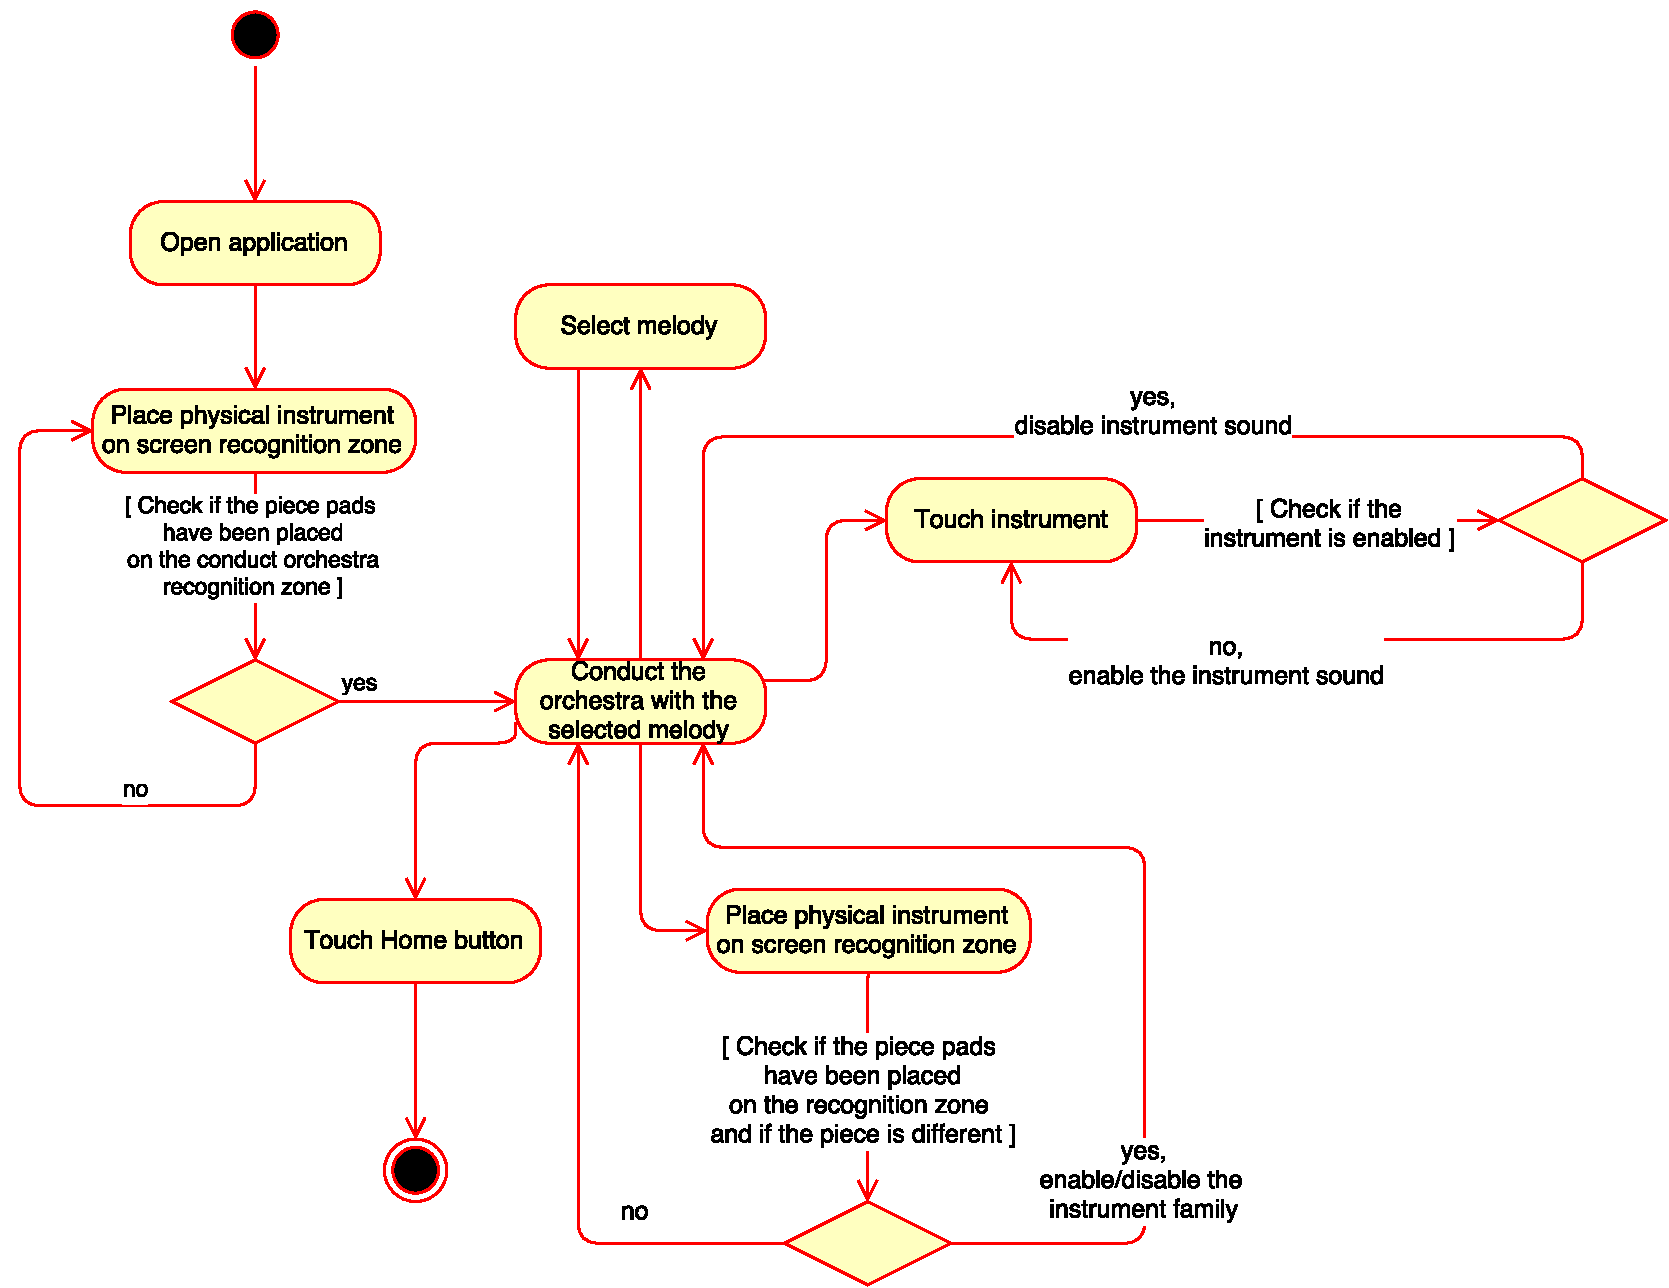
\includegraphics[width=400pt]{graphics/architecture/ConductingGameMode.pdf}
	\caption{Conducting orchestra game mode}
	\label{fig:conductingworkflow}
\end{figure}

As we can see in Figure \ref{fig:conductingworkflow}, to access \textit{Discovering instrument}, the gamer has to place the physical instrument miniature in the Discovering mode recognition zone after opening the application. If the instrument has been placed properly, the \textit{Discovering instrument} screen is opened.

Within this \textit{Discovering instrument} screen, the gamer can read information and learn about some instruments of the family instrument that has been placed to access the game mode. Also, the instrument sound can be reproduce touching the instrument sound button.

Also, the gamer is able to change the instrument by placing another instrument miniature on the instrument recognition zone.

Finally, the gamer can go back to the home screen touching the home button.

\FloatBarrier

\newpage
\subsection{Discovering instrument game mode}
\label{subsec:discoverinstrument_arch}

Discovering instrument game mode workflow is represented in Figure \ref{fig:discoveringworkflow}

\begin{figure}[ht!]
	\centering
	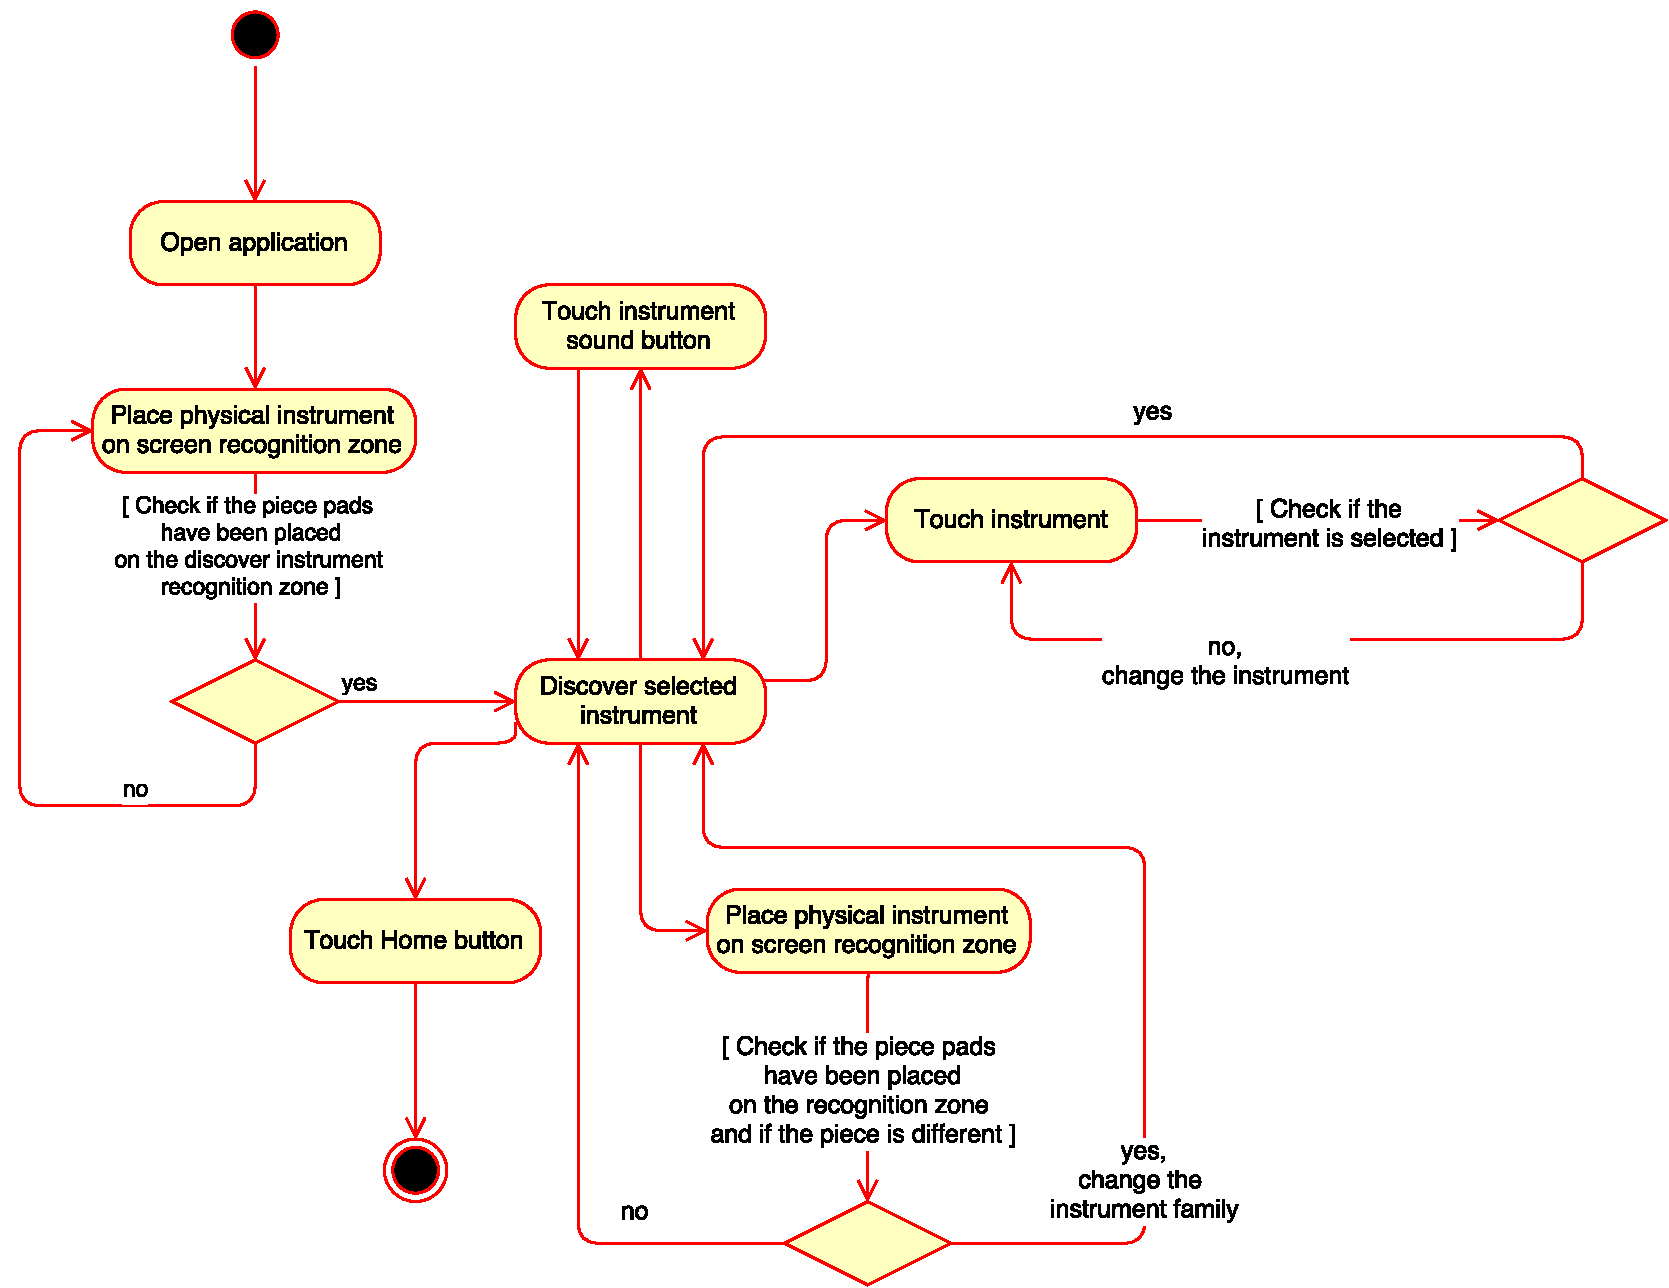
\includegraphics[width=400pt]{graphics/architecture/DiscoveringGameMode.pdf}
	\caption{Discovering instrument game mode}
	\label{fig:discoveringworkflow}
\end{figure}

As we can see in Figure \ref{fig:conductingworkflow}, to access \textit{Conducting the orchestra}, the gamer has to place the physical instrument miniature in the Conducting mode recognition zone after opening the application. If the instrument has been placed properly, the \textit{Conducting orchestra} screen is opened.

Within this \textit{Conducting orchestra} screen, the gamer can conduct an orchestra which is playing the selected melody. This melody can be changed by the gamer using the melody selector menu, that is shown after touching the melody button.

When this game mode is opened, the melody start to be played with all the instrument enabled. The gamer is able to enable or disable an instrument sound. Also, the gamer can enable or disable an entire family instrument placing one of the physical instrument miniatures in the instrument recognition zone.

\FloatBarrier

\section{Summary}
In this chapter, we presented the proposed architecture for our application.

We started by taking a look at the architecture overview, where we differentiated two principal components, the physical instruments miniatures and the software application.

After introducing both principal components, we saw how these physical instruments miniatures were designed and how they are recognized by the software application using a recognition algorithm.

Later, we detailed the software application architecture, focusing on how Unity3D engine and its assets as long as other components work together.

Finally, we described the three application game modes workflow.
